\documentclass[preprint,12pt]{elsarticle}
\ifdefined\pdfminorversion\pdfminorversion=7\fi
\usepackage[T1]{fontenc}
\usepackage[utf8]{inputenc}
\usepackage{lmodern,amsmath,amssymb,booktabs,array,graphicx}
\usepackage[margin=25mm]{geometry}
\usepackage{microtype,tikz,pgfplots}
\usetikzlibrary{arrows.meta,positioning}
\pgfplotsset{compat=1.18}
\usepackage[colorlinks=true,linkcolor=blue!45!black,citecolor=blue!45!black,urlcolor=blue!45!black]{hyperref}
\usepackage{caption}
\usepackage{pdflscape,longtable}
\captionsetup{font=small,labelfont=bf}
\setlength{\parskip}{4pt}
\setlength{\parindent}{1em}
\setlength{\emergencystretch}{2em}
\newcommand{\pos}[1]{[#1]_{+}}
\newcommand{\R}{\mathbb{R}}
\newcommand{\ind}{\mathbf{1}}
\journal{Electric Power Systems Research}
\begin{document}
\begin{frontmatter}
\title{Causal Trust Gating for Battery Dispatch in Distribution Networks under Degraded Measurements}
\author[upes]{Chandrasen Pandey\corref{cor}}
\cortext[cor]{Corresponding author.}
\ead{chandrasen.pandey@ddn.upes.ac.in}
\affiliation[upes]{organization={School of Computer Science, University of Petroleum and Energy Studies}, addressline={P.O. Bidholi, via Prem Nagar}, city={Dehradun}, postcode={248007}, state={Uttarakhand}, country={India}}
\begin{abstract}
Measurement quality can change the physical value of battery dispatch in a distribution-network digital twin. A causal supervisory gate combines observation age, availability, completed forecast performance and independent meter agreement to select full power, half power or a hold. Candidate and issued commands receive AC power-flow checks at the predicted state, while realised outcomes are evaluated separately. Fourteen controllers compare evidence scores, action policies, reference failures and finite-scenario uncertainty screening. Two rolling forecast origins and twenty-four temporal blocks cover an IEEE 33-bus feeder and aggregate and asset-specific representations of a 97-bus SimBench network, producing 1,959,552 controller records. Composite three-regime gating reduces violation rates relative to ungated dispatch from 0.442\% to 0.182\%, from 0.291\% to 0.135\%, and from 22.306\% to 21.725\%, respectively. Mean energy-adjusted cost rises by EUR 26.22, EUR 138.83 and EUR 25.08 per 72-hour block. An always-half policy gives lower observed violation rates and lower cost than the composite gate in all three representations. Composite evidence improves common-proposal ranking over agreement at 50\% and 75\% coverage only in the asset-specific case. Retrospective AC checks find a feasible tested power level in every realised state, but battery energy bounds exclude all such levels during 6,610 composite-gate failures in that case. The results support conditional use of evidence gating and show that action restriction, spatial operating profiles and energy headroom must be assessed together.
\end{abstract}
\begin{keyword}
Digital twin \sep Distribution network \sep Battery dispatch \sep Measurement quality \sep Forecast uncertainty \sep Power flow
\end{keyword}
\end{frontmatter}
\section{Introduction}\label{sec:intro}
Distribution networks with local generation and battery storage require control decisions that remain useful when measurements are incomplete, delayed or inconsistent. A digital twin can combine a network model with forecasts and operating records to support these decisions. The value of this combination depends on the information available when a command is issued. A forecast can appear accurate in an offline assessment while providing poor support for a particular dispatch decision. The resulting problem concerns both measurement quality and the physical consequences of control.

Storage introduces a further dependence across decision hours. A command changes both the present network injection and the energy available for later support. Restricting a recommendation can therefore alter later feasibility even when the restricted command is zero. This dependence makes it necessary to evaluate complete battery trajectories as well as individual proposals. It also prevents the fraction of authorised hours from serving as a substitute for useful control activity.


Digital twins for energy systems address modelling, data exchange and computational coordination \cite{ardebili}. Recent work has demonstrated a hardware-in-the-loop twin for analysing anomalies in a photovoltaic, hydrogen and storage system \cite{hueros}. Such developments establish the relevance of a digital representation connected to operating data. A separate requirement arises when the representation is used to authorise an action: evidence about the current data must be available before the action, and the resulting network state must be assessed independently.

Field-connected distribution twins already combine data collection, state estimation and flexibility assessment, as demonstrated by Bragatto et al. \cite{bragatto}. Muhsen et al. \cite{muhsen} connect distribution flexibility with measurement-attack detection and reconstruction for electric vehicle aggregators. These studies establish that data assurance and flexible-resource operation can be developed within a common twin. The present problem concerns a narrower decision: whether an already formed battery recommendation should be executed at full power, reduced power or zero power when the available measurement evidence deteriorates.


\subsection{Operational problem and research question}
Measurement faults can affect dispatch through several paths. Missing observations remove recent information, delayed observations describe an earlier state, and biased observations can produce an apparently plausible forecast of the wrong operating condition. An alternating-current (AC) power-flow check based on that forecast can therefore approve a command that violates limits in the actual network. Conversely, a gate that holds the battery whenever information deteriorates can remove useful voltage support. The quality of the gate cannot be inferred from its own authorisation rule.

The research question is whether combining measurement age, availability, completed forecast performance and meter agreement improves battery dispatch beyond a simpler consistency score and a cautious action policy. Two effects require separate assessment: the information supplied by the score and the operating effect of reducing battery power. A factorial comparison applies agreement and composite evidence to the same binary and three-regime policies. Reference failures and a reference-fed forecast also test whether the additional meter is being used effectively. Physical violations, cost and retained control provide the common basis for these comparisons.

\subsection{Scope and contributions}
The proposed method separates prediction, evidence scoring, command checking and plant evaluation. Every score uses current metadata or completed past observations. Battery commands are ranked with a local network approximation and checked against the alternating-current model before issue. A scaled command receives a further check because reduced battery power does not necessarily preserve feasibility. Holding the battery remains an explicit operating action whose physical consequences are recorded.

The study contributes a causal supervisory dispatch sequence, a paired evaluation that separates evidence scoring from action restriction, and a reproducible assessment across seasonal and spatial operating conditions. The comparison contains fourteen controller configurations, including four channel-removal controls, a reference-fed predictor and uncertainty-aware command screening. Two rolling forecast origins and twenty-four non-overlapping temporal blocks test an IEEE 33-bus feeder and a 97-bus SimBench network. The SimBench assessment includes both aggregate-factor operation and the original asset-specific profiles. The contribution is an applied dispatch method and its operational assessment. The random forest, split calibration and power-flow solver retain their established roles. The following literature discussion connects those roles to the control problem.

\subsection{Paper organisation}
Section~\ref{sec:related} examines the related work and defines the role of the proposed dispatch layer. Section~\ref{sec:model} introduces the information boundary, electrical constraints and battery objective. Section~\ref{sec:method} develops prediction, evidence scoring and command selection. Section~\ref{sec:experiments} describes the networks, chronological partitions, measurement conditions and evaluation measures. Section~\ref{sec:results} presents prediction and dispatch outcomes, followed by their operating implications and limitations in Section~\ref{sec:discussion}. Section~\ref{sec:conclusion} states the conclusions and remaining validation needs. Appendix~\ref{sec:checks} records the implementation checks supporting reproducibility.


\section{Related work and methodological position}\label{sec:related}
Three bodies of research inform the proposed dispatch method: digital twins that organise operating models, uncertainty-aware energy management, and the assessment of unreliable measurements. Their roles differ within a control pipeline. Distinguishing these roles provides a direct basis for selecting the comparison methods and evaluation measures.

\subsection{Digital twins and energy management}
The review by Aghazadeh Ardebili et al. \cite{ardebili} identifies design, management and computational challenges in energy-system twins. Zhang et al. \cite{zhang} study sequential optimisation in a digital-twin setting. These works motivate the integration of evolving information with decisions, while the present study concentrates on the point at which a battery recommendation is authorised. The implemented twin consists of a fixed electrical network model, an hourly state estimate, a next-hour predictor and a dispatch record. Its connection to a physical installation is emulated by separate measurement and plant streams.

The distribution-network case study of Bragatto et al. \cite{bragatto} integrates data collection, state estimation and a flexibility calculator with an existing network and reports a month of continuous operation. That field evidence concerns service integration and the calculation of available flexibility. The EV-aggregator framework of Muhsen et al. \cite{muhsen} includes detection and reconstruction of corrupted measurements. The present benchmark does not reproduce either field deployment or reconstruction method. It instead evaluates an observable authorisation rule on common storage recommendations, retaining the physical outcome of every issued action, including holds.


Panda et al. \cite{panda} compare approaches for handling uncertainty in real-time operation of a connected microgrid. Rahman and Ganguly \cite{rahman} use a reduced-model, dual-stage predictive controller for voltage regulation and loss reduction. These approaches address the control problem directly, including the use of forecasts and network constraints. The proposed gate can be examined alongside such controllers, but the implemented dispatch kernel is a one-step candidate search. Its performance is assessed within that kernel rather than attributed to a multi-period optimal control method.

Khojasteh et al. \cite{khojasteh} formulate energy and reserve provision for communities with shared storage using bounded forecast deviations and affine recourse rules. Their uncertainty budget controls the conservatism of an adaptive robust optimisation problem. In the present method, uncertainty calibration supplies residual evidence and the gate adjusts a checked point-forecast action. No worst-case network optimisation over an uncertainty set is solved. The comparison of these roles identifies where a gate could complement a more advanced controller without treating a residual score as robust recourse.


Hou et al. \cite{hou} combine behavioural learning, ensemble prediction and extended price forecasting in an uncertainty-informed twin for long-duration storage. Their objective concerns multi-day market dispatch. The hourly distribution-network problem considered here instead asks how current measurement evidence should modify a physically checked battery recommendation. This distinction concerns the decision horizon and evaluation loss, rather than the general use of prediction within a twin.

\subsection{Forecast uncertainty and downstream performance}
Forecast error and control loss are related but distinct. Li et al. \cite{li} demonstrate that the economic impact of storage-control forecast errors depends on the pricing scheme and error direction. This observation supports the use of operating outcomes rather than forecasting accuracy alone.

Sharma et al. \cite{sharma} examine battery-level mitigation of energy forecast errors in renewable microgrids and show the relevance of receding-horizon and regularised dispatch. Gadari and Kiran \cite{gadari} derive operational voltage flexibility from injection sensitivities and adjust the base optimisation problem to accommodate forecast errors. Both studies connect uncertainty to electrical or storage operation. They motivate two controls used here: always reducing a checked recommendation to half power, and checking a recommendation against four calibrated load-generation stress states. These controls test the value of caution without requiring a composite score.

Elmachtoub and Grigas \cite{elmachtoub} formalise this distinction through a loss based on the downstream optimisation decision. Paredes et al. \cite{paredes} apply decision-focused training to storage participation in reserve markets, incorporating the consequences of market decisions into prediction. Those methods change how the predictor is trained. Here the random forest remains fixed and the dispatch outcomes assess a separate authorisation layer. The distinction explains why lower forecast error alone cannot establish the benefit of the gate, and why feasibility, cost and retained control are reported together.
 A random forest supplies the point forecasts in the present study \cite{breiman}. A split-calibrated prediction box supplies a joint residual threshold for the two aggregate operating factors \cite{angelopoulos}.

The calibration procedure requires careful interpretation for hourly energy data. Exchangeability is a central condition in standard conformal analysis. Oliveira et al. \cite{oliveira} develop results for non-exchangeable processes under additional assumptions. Those assumptions are not established for the benchmark sequence used here. Accordingly, coverage is measured empirically and contributes an operating indicator. It is not treated as a guarantee that a selected dispatch command will satisfy network limits. Adaptive calibration under distribution shift is a further direction described by Gibbs and Cand\`es \cite{gibbs}.

\subsection{Unreliable measurements and decision evaluation}
False-data injection against grid state estimation can exploit relationships among measurements and the network model \cite{liu}. Detection and identification also depend on the structure of the monitored cyber-physical system \cite{pasqualetti}. The bias experiment in this study is an explicit corruption of operating measurements. It tests dispatch sensitivity and does not represent a stealth attack designed to bypass a state estimator.

Shen et al. \cite{shen} evaluate anomalous physical-twin data through detection, localisation and estimation before updating a power-system twin. Their data-assurance layer addresses unreliable model updates. The proposed gate acts after prediction and candidate selection, and does not reconstruct measurements. The distinction is necessary because a low evidence score can restrict an action while leaving the underlying forecast error unchanged. Common bias in both meters provides a direct test of this limitation.

Recent work on low-voltage topology correction also shows that data quality and network-model accuracy remain linked in a digital-twin setting \cite{dongliu}. The present experiments hold topology and electrical parameters fixed. They isolate the effects of operating-data quality, so their conclusions do not extend to undetected topology errors.

Gao et al. \cite{gao} address topology identification under asynchronous low-voltage meter sampling by imposing physical structure on coupling-impedance estimation. Their work illustrates that timing inconsistency can affect network inference even when individual readings are plausible. The present delay experiment instead changes the operating-factor features supplied to a fixed network model. Neither topology reconstruction nor state-estimator attack detection is evaluated. Risk-coverage analysis \cite{geifman} supplies a useful selection framework for examining the score, provided that its loss is defined by the realised constraint outcome rather than imported from a different prediction task.
 Table~\ref{tab:position} summarises the methodological position. This distinction leads to the formal description of information, network constraints and battery state in the next section.

\begin{table}[t]
\centering\small
\caption{Position of the dispatch study relative to selected research directions.}\label{tab:position}
\begin{tabular}{>{\raggedright\arraybackslash}p{.23\linewidth}>{\raggedright\arraybackslash}p{.30\linewidth}>{\raggedright\arraybackslash}p{.37\linewidth}}
\toprule
Research direction & Main role & Role in the present study\\
\midrule
Energy-system twins \cite{ardebili,hueros,zhang} & Model and operating-data integration & Emulated state synchronisation and command records\\
Uncertain energy management \cite{panda,rahman,li} & Forecast-informed control and operating objectives & Common dispatch kernel for all gates\\
Conformal prediction \cite{angelopoulos,oliveira,gibbs} & Prediction-set calibration & Empirical joint residual indicator\\
Measurement attacks \cite{liu,pasqualetti} & Detection and identifiability & Observable meter agreement and a defined bias test\\
Topology correction \cite{dongliu} & Network-model consistency & Fixed-topology boundary of the experiments\\
\bottomrule
\end{tabular}
\end{table}

\section{System model and information structure}\label{sec:model}
The dispatch problem is defined on a distribution network with fixed loads, distributed generation and one controllable battery. The model distinguishes the estimated next-hour state from the plant state that becomes known after a command. This distinction is maintained in both the equations and the implementation.

\subsection{Decision-time information}
Let $y_t$ denote the vector of operating factors at hour $t$. In the aggregate experiments, $y_t=(\ell_t,g_t)^{\mathsf T}$ contains load and generation factors. In the asset-specific experiment, $y_t\in\R^{32}$ contains ten active-load, ten reactive-load and twelve generation profile factors. Index $t$ identifies the latest observed hourly state, and command $u_t$ applies to the next hourly operating state. The dimensionless factors multiply the corresponding installed active or reactive powers in the network. The primary observation is $z_t$, the separately measured reference is $r_t$, the observation-age metadata is $a_t$, the primary availability indicator is $m_t\in\{0,1\}$, and the reference availability indicator is $n_t\in\{0,1\}$. An observation that is missing is replaced by the last available primary observation. This forward carry uses no later value.

The information available to the controller is
\begin{equation}
\mathcal F_t=\sigma\{z_s,r_s,a_s,m_s,n_s,u_{s-1},x_s:s\leq t;\ \theta,\mathcal D_{\mathrm{train}},\mathcal D_{\mathrm{cal}},\mathcal D_{\mathrm{dev}}\},
\label{eq:information}
\end{equation}
where $u_t$ is battery power, $x_t$ is state of charge, and $\theta$ contains fixed model and control parameters. The next-hour plant state $y_{t+1}$ and injected-fault labels are excluded from $\mathcal F_t$. A command must be a function of $\mathcal F_t$. The evaluator later receives $y_{t+1}$ to calculate the operating outcome. The reference stream is available at the current hour and is used to assess past forecasts and current meter agreement; it is not a next-hour oracle.

The information structure creates two clocks. At the decision clock, measurements through hour $t$ can complete the assessment of a forecast issued at $t-1$. The forecast issued at $t$ remains unassessed until the next reference observation arrives. At the outcome clock, the evaluator applies the issued command to the realised next-hour injections. Maintaining these clocks separately avoids assigning a low score to a forecast using information that was unavailable when its command was selected.

The stored battery state is controller specific, whereas operating factors, measurement corruptions and tariffs are shared within a paired experiment. Consequently, identical scores can produce different proposals after the controllers have followed different trajectories. The reference is an additional information source whose reliability is tested explicitly. The proposed gate uses it for current consistency and completed performance evidence. A comparison predictor receives its current and past readings instead of the primary features, with primary-predictor fallback during an outage. Neither use reveals the next-hour plant state. Keeping these alternatives explicit tests the operational value of evidence gating against direct use of the additional meter.


\subsection{Electrical network}
For buses $i,j\in\mathcal N$, let $Y_{ij}=G_{ij}+\mathrm jB_{ij}$ denote the per-unit bus-admittance entries, $V_i$ the per-unit voltage magnitude and $\delta_{ij}$ the angle difference in radians. Let $S_B$ be the benchmark apparent-power base in MVA. Active and reactive injections $P_i$ and $Q_i$ are expressed in MW and MVAr. The balanced, steady-state power-flow equations are
\begin{align}
P_i&=S_BV_i\sum_{j\in\mathcal N}V_j\big(G_{ij}\cos\delta_{ij}+B_{ij}\sin\delta_{ij}\big),\label{eq:acp}\\
Q_i&=S_BV_i\sum_{j\in\mathcal N}V_j\big(G_{ij}\sin\delta_{ij}-B_{ij}\cos\delta_{ij}\big).\label{eq:acq}
\end{align}
At the battery bus $b$, positive $u_t$ represents discharge and increases active injection. In the aggregate experiments, loads retain their benchmark power factors as $\ell_t$ changes. Asset-specific reactive-load factors are represented separately below. Distributed generators and the battery operate at unity power factor. The grid interconnection supplies the remaining active and reactive power. For non-slack buses, the next-hour injections are
\begin{equation}
P_{i,t+1}=g_{t+1}P_i^G-\ell_{t+1}P_i^L+\ind\{i=b\}u_t,\qquad
Q_{i,t+1}=-\ell_{t+1}Q_i^L,\quad i\ne s,
\label{eq:injections}
\end{equation}
where $P_i^G$, $P_i^L$ and $Q_i^L$ are installed generation, active load and reactive load, and $s$ is the slack bus. The model check replaces the realised factors in Eq.~\eqref{eq:injections} with their next-hour forecasts. Voltage and thermal limits are
\begin{equation}
0.95\leq V_i\leq1.05,\qquad
\rho_e\leq1\quad(e\in\mathcal E),
\label{eq:limits}
\end{equation}
where $\rho_e$ is line-current utilisation or transformer apparent-power utilisation. The voltage band in Eq.~\eqref{eq:limits} is imposed uniformly for this study. The original SimBench bus limits include 0.90--1.10~p.u. and 0.965--1.055~p.u.; they are not used as the acceptance band in these experiments. Reported violations therefore concern the common study limits, rather than compliance with each native benchmark voltage band. Network feasibility requires convergence of Eqs.~\eqref{eq:acp}-\eqref{eq:acq} and satisfaction of all limits in Eq.~\eqref{eq:limits}. The implementation uses the benchmark network data and the pandapower solver \cite{baran,meinecke,thurner}.

Feasibility is a property of a particular operating state and action. Define $\mathcal A(y)=\{u:h(y,u)\text{ converges and satisfies Eq.~\eqref{eq:limits}}\}$, with $h$ denoting the AC network solution. The distinction between estimated and realised admissibility is then
\begin{equation}
u_t\in\mathcal A(\widehat y_{t+1|t})
\quad\not\Rightarrow\quad
u_t\in\mathcal A(y_{t+1}).
\label{eq:modelplant}
\end{equation}
The forecast check removes actions that are unsuitable in the estimated state. It does not bound the error between that state and the plant. Likewise, reducing the magnitude of an action does not generally preserve membership in $\mathcal A(y)$: a smaller discharge can remove voltage support needed at a weak bus. The gate therefore operates together with a second check of the actual command.


For the asset-specific network, fixed index maps $\pi_P(i)$, $\pi_Q(i)$ and $\pi_G(j)$ associate each load or generator with its supplied profile group. Its nodal inputs are
\begin{align}
p_{i,t}^{L}&=\bar p_i^{L}y_{t,\pi_P(i)}, & q_{i,t}^{L}&=\bar q_i^{L}y_{t,\pi_Q(i)},\label{eq:assetloads}\\
p_{j,t}^{G}&=\bar p_j^{G}y_{t,\pi_G(j)}.\label{eq:assetgeneration}
\end{align}
The bars denote installed powers. Profile maps remain fixed while factors vary independently across groups. The predictor estimates these factors before the AC check, and the evaluator subsequently applies their realised values. For a common evidence scale across experiments, $B(y)$ returns the installed-power-weighted active-load and generation factors:
\begin{equation}
B(y)=\left(\frac{\sum_i\bar p_i^{L}y_{\pi_P(i)}}{\sum_i\bar p_i^{L}},
\frac{\sum_j\bar p_j^{G}y_{\pi_G(j)}}{\sum_j\bar p_j^{G}}\right)^{\mathsf T}.
\label{eq:aggregation}
\end{equation}
In the aggregate experiments $B$ is the identity. Evidence calculated from $B$ can miss spatial discrepancies that cancel in the totals. This limitation is retained when interpreting the asset-specific outcomes. Battery dynamics introduce the temporal dependence that accompanies these nodal states.

\subsection{Battery and operating objective}
For interval $\Delta t=1$~h, capacity $E^{\max}$ in MWh and efficiencies $\eta_c=\eta_d=0.94$, the battery state satisfies
\begin{equation}
x_{t+1}=x_t+\frac{\Delta t}{E^{\max}}\left(\eta_c\pos{-u_t}-\frac{\pos{u_t}}{\eta_d}\right),\qquad
0.15\leq x_{t+1}\leq0.90,\quad |u_t|\leq P^{\max}.
\label{eq:soc}
\end{equation}
Here $\pos{v}=\max(v,0)$. Battery energy is $E_t=x_tE^{\max}$. State of charge is treated as a reliable local battery-management measurement. Its measurement errors and converter dynamics are outside the hourly supervisory model.

Equation~\eqref{eq:soc} gives explicit energy-dependent power limits at a known starting state:
\begin{align}
u_t^{\min}&=-\min\!\left\{P^{\max},
\frac{E^{\max}(0.90-x_t)}{\eta_c\Delta t}\right\},\label{eq:chargebound}\\
u_t^{\max}&=\min\!\left\{P^{\max},
\frac{\eta_dE^{\max}(x_t-0.15)}{\Delta t}\right\}.\label{eq:dischargebound}
\end{align}
For $x_t\in[0.15,0.90]$, the interval $[u_t^{\min},u_t^{\max}]$ contains zero. Scaling an energy-admissible action toward zero therefore preserves battery admissibility. This property concerns the battery bounds alone. The voltage and thermal conditions still require an AC check, including when the proposed action is a hold.


Let $p_{t+1}^{\mathrm{grid}}(u)$ be the next-hour grid power under command $u$, positive for import, and let $c_{t+1}^{\mathrm{buy}}$ be the known tariff for that hour. The one-hour operating objective, in euros, is
\begin{equation}
J_t(u)=\Delta t\left(c_{t+1}^{\mathrm{buy}}\pos{p_{t+1}^{\mathrm{grid}}(u)}
-c^{\mathrm{sell}}\pos{-p_{t+1}^{\mathrm{grid}}(u)}+c^{\mathrm{deg}}|u|\right)
-c^{\mathrm{store}}(E_{t+1}-E_t).
\label{eq:cost}
\end{equation}
The last term values the change in stored energy and allows trajectories with different terminal states to be compared. It does not impose a terminal state constraint. The assumed buying prices are 70~EUR/MWh during hours 00:00-06:59, 240~EUR/MWh during 17:00-21:59, and 150~EUR/MWh otherwise. Export receives 40~EUR/MWh, throughput costs 10~EUR/MWh, and stored energy is valued at 130~EUR/MWh. These fixed study tariffs isolate dispatch behaviour; they are not observations from an electricity market. The resulting model supplies the candidate actions on which the trust gate operates.

For a block of $H$ issued commands, the stored-energy terms telescope:
\begin{equation}
\sum_{t=0}^{H-1}J_t(u_t)=
\sum_{t=0}^{H-1}\Delta t\left(c_{t+1}^{\mathrm{buy}}\pos{p_{t+1}^{\mathrm{grid}}}
-c^{\mathrm{sell}}\pos{-p_{t+1}^{\mathrm{grid}}}+c^{\mathrm{deg}}|u_t|\right)
-c^{\mathrm{store}}(E_H-E_0).
\label{eq:blockcost}
\end{equation}
Thus the reported objective compares grid transactions and throughput after a common valuation of remaining energy. Ending with less energy incurs the corresponding terminal-energy debit at the specified valuation. The valuation is linear and fixed; its numerical choice can change the preferred charging times. The throughput term is a simplified operating charge and does not describe electrochemical degradation or a battery replacement schedule.


\section{Causal trust-gated dispatch}\label{sec:method}
The method first predicts the next-hour operating factors and forms a battery recommendation using the estimated network state. It then combines four pieces of available evidence to choose full dispatch, cautious dispatch or a hold. The complete sequence is shown in Fig.~\ref{fig:architecture}. The plant evaluator remains outside the authorisation path.

The gate uses a recommendation already screened by the physical model. Quality indicators determine how much of that recommendation may be executed, while the final model check determines whether the resulting command is admissible in the predicted state. This ordering makes the architecture inspectable: each recorded decision identifies the information used, the original proposal, the selected regime and the issued action. The construction below describes these components before combining them into one decision sequence.


\clearpage
\newgeometry{margin=12mm}
\begin{landscape}
\begin{figure}[p]
\centering
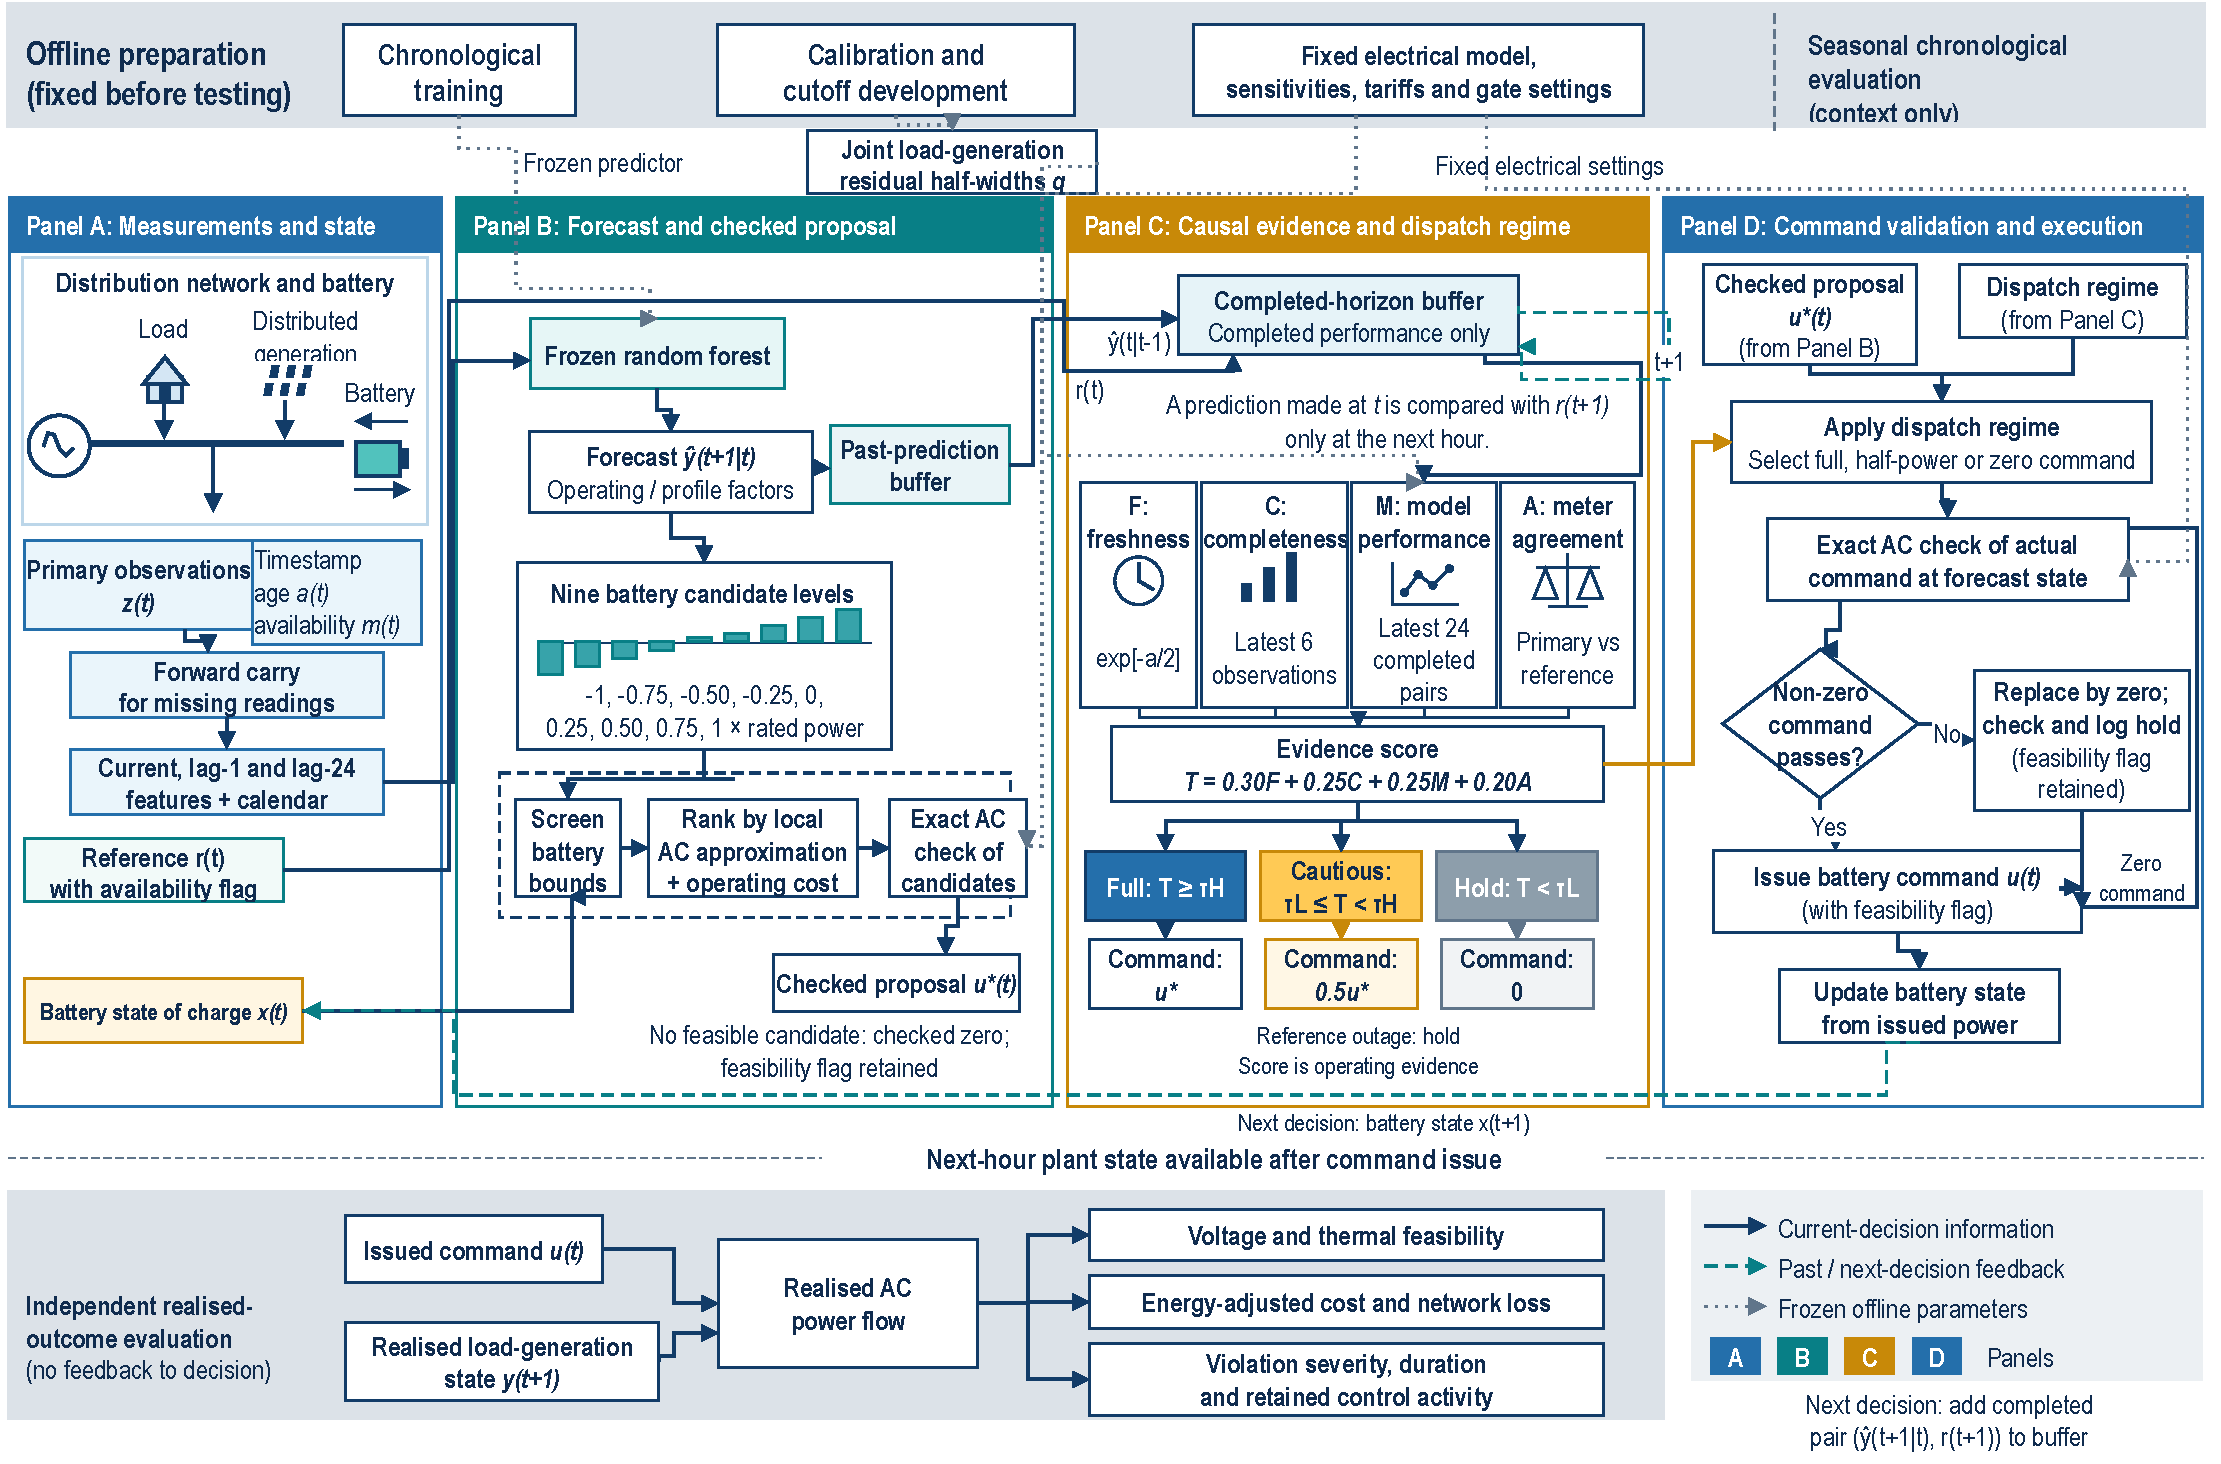
\includegraphics[width=245mm,height=164mm,keepaspectratio]{epsr_figures/Figure_1.pdf}
\caption{Causal architecture of trust-gated battery dispatch. Panel A supplies primary measurements, reference observations and battery state. Panel B forms an AC-checked proposal from a frozen predictor. Panel C combines freshness, completeness, completed forecast performance and meter agreement into full, cautious or hold dispatch. Panel D checks the actual command before issue and updates battery state. Realised next-hour outcomes remain outside the current authorisation path; reference feedback enters only after its forecast horizon has ended.}\label{fig:architecture}
\end{figure}
\end{landscape}
\restoregeometry


\subsection{Point prediction and joint residual calibration}
The feature vector contains $z_t$, $z_{t-1}$, $z_{t-24}$, sine and cosine encodings of hour of day, and sine and cosine encodings of day of year. A multi-output random forest with 60 trees, minimum leaf size eight and feature fraction 0.75 predicts
\begin{equation}
\widehat y_{t+1|t}=f_{\theta}(z_t,z_{t-1},z_{t-24},\mathrm{calendar}_t).
\label{eq:forecast}
\end{equation}
Negative predictions are clipped to zero. The model is fitted on the training partition for each rolling origin; its parameters remain fixed throughout its calibration, development and test periods.

Let $s_j>0$ be the 90th percentile of absolute training residuals for coordinate $j\in\{\ell,g\}$ of $B(y)$, with a lower bound of $10^{-6}$. For calibration observations indexed by $i$, define
\begin{equation}
e_i=\max_{j\in\{\ell,g\}}\frac{|B(y_{i+1})_j-B(\widehat y_{i+1|i})_j|}{s_j},\quad
k=\min\{n_{\mathrm{cal}},\lceil(n_{\mathrm{cal}}+1)(1-\alpha)\rceil\},\quad \alpha=0.10.
\label{eq:calibration}
\end{equation}
If $e_{(k)}$ is the $k$th ordered calibration residual, the joint box is
\begin{equation}
\mathcal I_t=\prod_{j\in\{\ell,g\}}
[B(\widehat y_{t+1|t})_j-q_j,B(\widehat y_{t+1|t})_j+q_j],\qquad q_j=s_je_{(k)}.
\label{eq:interval}
\end{equation}
This is the standard split-calibration construction applied to a maximum residual \cite{angelopoulos}. It supplies a common joint exceedance test. Its observed coverage is reported because serial dependence and seasonal change affect interpretation \cite{oliveira}.

Taking the maximum normalised residual makes exceedance a joint event: a calibration pair lies inside the box only when both load and generation errors are within their respective half-widths. The training scales place the two coordinates on comparable residual units, and the calibration quantile then adjusts their common multiplier. The resulting box is used to assess completed prediction residuals. Candidate acceptance is evaluated at the point forecast, rather than over every state inside the box. Therefore prediction coverage, model feasibility and realised feasibility remain separate quantities.

Freezing the predictor and half-widths before testing prevents a controller from using the reported test outcomes to improve its forecasts retrospectively. This design also exposes changes in seasonal performance. A future implementation could update calibration sequentially using completed observations, following the distribution-shift setting considered by Gibbs and Cand\`es \cite{gibbs}, but such updating is outside the tested policy.


\subsection{Observable evidence channels}
Four channels measure different aspects of the available information. Freshness is $F_t=\exp(-a_t/2)$, with age measured in hours. Completeness is $C_t=\frac{1}{6}\sum_{s=t-5}^{t}m_s$, the fraction of primary observations available during the latest six hours. Both indicators follow from stream metadata.

Recent model performance is evaluated against reference observations whose forecast horizons have already ended. For at most 24 completed pairs in $\mathcal H_t$, define
\begin{align}
\widehat c_t&=\frac{1}{|\mathcal H_t|}\sum_{s\in\mathcal H_t}
\ind\{\max_j|B(r_s)_j-B(\widehat y_{s|s-1})_j|/q_j\leq1\},\label{eq:recentcoverage}\\
\widehat d_t&=\frac{1}{2|\mathcal H_t|}\sum_{s\in\mathcal H_t}\sum_j
|B(r_s)_j-B(\widehat y_{s|s-1})_j|,\label{eq:recentmae}\\
M_t&=\frac{1}{2}\min\{1,\widehat c_t/0.90\}
+\frac{1}{2}\exp[-\widehat d_t/(3d_{\mathrm{cal}})].\label{eq:maturity}
\end{align}
Here $d_{\mathrm{cal}}$ is the mean absolute calibration error averaged over both factors. At block initialisation, $\widehat c_t=0.90$ and $\widehat d_t=d_{\mathrm{cal}}$. Subsequent values use the latest 24 completed pairs with received reference observations; an outage does not add a carried reference value to this history. Thus a forecast made at $t$ cannot be evaluated against $r_{t+1}$ while selecting $u_t$.

Agreement between the current primary and reference measurements is
\begin{equation}
A_t=\exp\left[-\frac{|B(z_t)_\ell-B(r_t)_\ell|+|B(z_t)_g-B(r_t)_g|}{2\kappa}\right],\qquad\kappa=0.10.
\label{eq:agreement}
\end{equation}
Independent reference noise is the nominal condition. During a reference outage, $A_t=0$ and all reference-dependent gates select a hold. The forecast baseline instead uses the primary predictor for that decision. No carried reference value is treated as a fresh agreement observation. The common-bias condition deliberately violates meter independence, so agreement alone cannot establish source authentication.

The operating evidence score is
\begin{equation}
T_t=0.30F_t+0.25C_t+0.25M_t+0.20A_t.\label{eq:trust}
\end{equation}
All channels lie in $[0,1]$, so the score is bounded by the same interval. The channel weights and scale constants are fixed design choices. The operating cutoffs are fitted on development scores to prescribed coverage targets. A separate fixed-cutoff control retains $0.65$ and $0.85$. The score has no probability interpretation. Channel-removal controls and common-proposal ranking assess the information supplied by the components.

The channels respond on different time scales. Freshness reacts to current age, agreement reacts to current inconsistency, completeness summarises six hours, and model performance summarises up to 24 completed horizons. A physical disturbance visible to both meters can preserve agreement while increasing recent forecast errors. Conversely, corruption confined to the primary meter can lower agreement immediately. The score combines these observable effects without identifying the cause of a low value.

Some regime effects follow directly from the specified weights. For a two-hour-old observation, the fixed-cutoff score satisfies the following bound even with perfect values of the other channels:
\begin{equation}
T_t\leq0.30\exp(-1)+0.25+0.25+0.20=0.81036<0.85.
\label{eq:delaybound}
\end{equation}
The delayed condition can therefore receive cautious dispatch or a hold, but never full dispatch under the fixed-cutoff rule. One missing observation in a six-hour window reduces the completeness contribution by $0.25/6=0.04167$ before any age or agreement effect. At block initialisation, the model-performance prior yields $M_t=0.5+0.5\exp(-1/3)=0.85827$; it is replaced progressively by completed pairs. These algebraic properties explain the behaviour imposed by the design and are distinct from empirical evidence of improved network operation.


\subsection{Candidate ranking and command checks}
The action set is $\mathcal U_t=\{rP^{\max}:r=-1,-0.75,\ldots,1\}$ after removing actions that violate Eq.~\eqref{eq:soc}. A local approximation of the AC solution is used for ranking. If $h(y,u)$ stacks bus voltages, branch utilisation, grid power and losses, then
\begin{equation}
\widetilde h(y,u)=h(y^0,0)+H_y(y-y^0)+H_u u.\label{eq:linear}
\end{equation}
The aggregate expansion point is $y^0=(0.6,0.4)^{\mathsf T}$. For the asset case, $y^0$ is the coordinate-wise median of the training and calibration periods, fixed before development and testing. The sensitivities are calculated with separate forward perturbations of $10^{-3}$ in each factor and $10^{-3}$~MW in battery power. The approximation is fixed before testing. It uses network parameters rather than the latent next-hour plant state.

Let $v(h)$ denote the non-negative aggregate limit excess,
\begin{equation}
v(h)=\pos{0.95-\min_i V_i}+\pos{\max_i V_i-1.05}
+\pos{\max_e\rho_e-1}.\label{eq:severity}
\end{equation}
Actions are ranked by $\widetilde J_t(u)+10^5v(\widetilde h)$, where $\widetilde J_t$ uses the approximate grid power in Eq.~\eqref{eq:cost}. The first action in this order that passes the exact AC check at $\widehat y_{t+1|t}$ is the proposal $u_t^\star$. If no candidate passes, the proposal is zero and the feasibility of that hold is recorded. This finite search provides a checked recommendation; its coarse action grid and approximate ranking do not establish a global optimum.

For development-fitted thresholds $\tau_L$ and $\tau_H$, the gated command is
\begin{equation}
\bar u_t=\begin{cases}
0,&n_t=0,\\
u_t^\star,&n_t=1,\ T_t\geq\tau_H,\\
0.5u_t^\star,&n_t=1,\ \tau_L\leq T_t<\tau_H,\\
0,&n_t=1,\ T_t<\tau_L.
\end{cases}\label{eq:regimes}
\end{equation}
The AC check is applied to $\bar u_t$ before it is issued. A non-zero command that fails this check is replaced by zero, and that hold is checked and logged. State of charge is updated only after command selection. A model-feasible command can still fail in the plant because $\widehat y_{t+1|t}\ne y_{t+1}$. This remaining error is the reason for independent evaluation.

Table~\ref{tab:algorithm} assembles the causal sequence. The full-power proposal and half-power command are separate objects. A half-power value can lie between two members of the original candidate grid, which is why its AC result cannot be inferred from the proposal check. The zero fallback is retained with its feasibility flag even when no feasible candidate exists. An operational record can therefore distinguish a model-feasible zero action from a hold issued in an infeasible estimated state.

\begin{table}[t]
\centering\small
\caption{Decision sequence for the trust-gated controller at hour $t$. The outcome step is isolated from command selection.}\label{tab:algorithm}
\begin{tabular}{>{\raggedright\arraybackslash}p{.08\linewidth}>{\raggedright\arraybackslash}p{.82\linewidth}}
\toprule
Step & Operation and information used\\\midrule
1 & Read $z_t,r_t,a_t,m_t,n_t,x_t$; carry forward a missing primary observation and construct current and past features.\\
2 & Append the completed pair $(\widehat y_{t|t-1},r_t)$ when available; retain the latest 24 completed pairs.\\
3 & Form $\widehat y_{t+1|t}$ with the frozen predictor; calculate $F_t,C_t,M_t,A_t$ and $T_t$.\\
4 & Screen nine candidate levels against battery bounds, rank the remaining actions and accept the first forecast-state AC-feasible proposal. Use a checked zero proposal if none passes.\\
5 & Apply the full, cautious or hold regime in Eq.~\eqref{eq:regimes}; recheck the resulting command with the forecast-state AC model.\\
6 & Replace a failed non-zero command by a checked hold; issue the command and retain its model-feasibility flag.\\
7 & Update battery state from the issued power; retain the proposal, channels, score, regime, command and state for the decision record.\\
8 & After the next-hour plant state is available, calculate realised AC outcomes, cost and evaluation measures. Make the next completed reference pair available only at the next decision.\\
\bottomrule
\end{tabular}
\end{table}


\subsection{Coverage calibration and comparison policies}
Let $\mathcal D_{\mathrm{dev}}$ contain development scores from the prescribed mixture of conditions and seeds, using hours with a received reference observation. For score $S\in\{A,T\}$, the cutoffs are
\begin{equation}
\tau_L^S=Q_{0.15}(S_t:t\in\mathcal D_{\mathrm{dev}},n_t=1),\qquad
\tau_H^S=Q_{0.50}(S_t:t\in\mathcal D_{\mathrm{dev}},n_t=1),
\label{eq:cutoffs}
\end{equation}
where $Q_p$ is the linearly interpolated empirical quantile. The targets are 85\% authorisation and 50\% full dispatch conditional on reference availability. Equality is retained, so tied scores can yield greater coverage. Test coverage is measured and need not equal its development target. No test feasibility or cost enters Eq.~\eqref{eq:cutoffs}.

The binary policy issues $u_t^\star$ if $n_t=1$ and $S_t\geq\tau_L^S$, and zero otherwise. The three-regime policy uses Eq.~\eqref{eq:regimes} with the same score. Crossing two scores with two policies separates the evidence representation from the power reduction rule. For removal of channel $j$, the retained score is
\begin{equation}
T_t^{(-j)}=\frac{\sum_{k\ne j}w_k E_{k,t}}{1-w_j},\qquad
(E_{1,t},E_{2,t},E_{3,t},E_{4,t})=(F_t,C_t,M_t,A_t).
\label{eq:ablation}
\end{equation}
Each removed-channel control receives its own development cutoffs at the same targets. The full experiment also retains the fixed-cutoff composite gate, so effects of coverage calibration remain observable.

\subsection{Reference prediction and uncertainty-aware screening}
The reference-fed control forms $f_\theta(r_t,r_{t-1},r_{t-24},\mathrm{calendar}_t)$ with the same trained random forest. Missing reference history is carried forward causally. If the current reference is missing, the primary forecast supplies that hour's candidate. This control uses a better meter directly when it is available; it does not receive a future observation.

The uncertainty-aware control tests a finite set of stress states rather than selecting an evidence regime. Let $\widetilde q_j$ be the 90th percentile of coordinate-wise absolute calibration errors in the operating-factor vector. Let $s_P$ and $s_G$ select load coordinates, including reactive-load coordinates, and generation coordinates. Its checked state set is
\begin{equation}
\mathcal S_t=\{\widehat y_{t+1|t}\}\cup
\{[\widehat y_{t+1|t}+\epsilon_P(s_P\odot\widetilde q)
+\epsilon_G(s_G\odot\widetilde q)]_+:
\epsilon_P,\epsilon_G\in\{-1,1\}\}.
\label{eq:stressstates}
\end{equation}
Here $\odot$ is coordinate-wise multiplication and clipping acts separately on each coordinate. A candidate must pass the AC check at every state in $\mathcal S_t$. Candidates retain the common point-state ranking and battery constraints. If none passes, a checked zero action is issued. The four perturbations represent jointly increasing or decreasing load and generation. They do not enumerate every corner of the 32-dimensional asset box, and checking corners does not bound interior nonlinear AC states. The comparison therefore supplies finite-scenario caution rather than a robust-feasibility certificate.

\subsection{Computational implementation}
Power-flow solutions are cached by operating factors and battery power within each fixed network. State-of-charge screening remains outside the cache because action admissibility depends on the individual controller trajectory. The cache changes computational reuse rather than the information supplied to the gate. A realised-state solution can be requested only after the command has been selected. The resulting records preserve the proposal, regime, command, starting state and physical outcome at each hour. This common execution structure allows the experiments to compare gates without changing the underlying dispatch kernel.

The candidate search requires at most nine candidate AC checks before a proposal is found or all admissible levels are exhausted. The actual-command check can reuse a previously evaluated full-power or zero action. A cautious value can require an additional solve, and a failed non-zero value can require a zero fallback check. This finite workload does not establish a bound on solver time or convergence. Offline sensitivities require a base solution and one perturbation for each of the two factors and battery power. They affect ordering only; no approximate solution is accepted in place of the specified AC feasibility test.

Evaluation adds realised-state solves and retrospective comparator actions. These calculations belong to the experiment harness and are not required to issue a live command. Keeping them outside the dispatch interface keeps the realised-action diagnostic and fault labels outside control inputs. This separation also allows a future predictor or dispatch kernel to be substituted while retaining the same causal scoring and outcome definitions.


\section{Experimental design}\label{sec:experiments}
The experiment applies the complete dispatch sequence to common measurements, forecasts and operating states. Controllers retain separate battery trajectories. Its factorial comparisons isolate score and policy choices, while the reference and spatial conditions test assumptions about the information supplied to the twin. The controller design and coverage targets were fixed before running the test experiments.

\subsection{Networks and operating profiles}
The IEEE 33-bus feeder follows the Baran--Wu benchmark \cite{baran}, with installed load 3.715~MW. Three unity-power-factor generators of 0.6~MW are added at zero-based buses 17, 24 and 32. A 0.8~MW, 3.2~MWh battery is connected at bus 17. The slack voltage is 1.0~p.u. A 0.4~kA current rating is imposed on each line because the supplied case does not contain usable thermal ratings. This is a study assumption rather than an original benchmark rating.

The rural MV SimBench case \texttt{1-MV-rural-{}-0-sw} contains 97 buses, 99 line entries, two transformers, 96 loads and 102 generators \cite{meinecke,dataset}. Its installed active load is 17.256~MW and generation is 25.565~MW. The original topology, switches, line ratings and transformer ratings are retained. A 2~MW, 8~MWh battery is connected at zero-based bus 15, the highest-voltage bus in the unprofiled initial benchmark solve. Slack voltage is 1.025~p.u. The two SimBench experiments use this same electrical network and storage placement.

The aggregate experiments use installed-power-weighted load and generation factors from the SimBench profiles, averaged over each group of four quarter-hour samples. These factors scale every load and generator in the IEEE feeder and in the aggregate SimBench case. The asset-specific SimBench experiment instead retains the original profile of every element through Eqs.~\eqref{eq:assetloads}--\eqref{eq:assetgeneration}. Ten active-load groups, ten reactive-load groups and twelve generation groups give a 32-dimensional operating vector. Each group receives its own next-hour forecast. Thus realised spatial diversity is also represented in the predicted network inputs; it is not inserted solely into the evaluator.

The profiles cover the 8,784 hours of leap year 2016. They are benchmark operating sequences, with simulated measurement faults, rather than measurements collected from a deployed twin. The storage efficiencies, limits and study tariffs are shared across cases. Battery state starts at 0.55 for each controller in each test block. This common reset supports paired block comparisons, while dependence within a block remains part of the operating response.

\subsection{Rolling origins and independent temporal blocks}
The summer origin trains on January--April, calibrates on May and sets coverage cutoffs on June. Its test blocks start on July 1, 5, 9, 13, 17, 21, 25 and 28. The winter origin trains on January--August, calibrates on September and sets cutoffs on October. Its blocks start on the same eight dates in both November and December. Every block contains 72 issued commands and 24 hours of causal prehistory. Training, calibration and development indices retain both the current observation and next-hour target inside their own partition.

These origins provide eight summer blocks and sixteen winter blocks. The 24 test blocks do not overlap. Their use does not imply that all hourly errors are independent; the statistical analysis preserves the complete physical block. The predictor and electrical sensitivities remain fixed for an origin, with electrical coefficients retained across the paired conditions. Each experimental condition receives the paired measurement seeds 11, 29 and 47. Seeds vary measurement corruption while the physical benchmark sequence remains common.

\subsection{Primary and reference measurement conditions}
Table~\ref{tab:conditions} specifies nine equally weighted conditions. Faults affect profile factors before features are constructed. In the aggregate cases they act on two coordinates; in the asset case they act on the 32 profile-group coordinates. Availability and age describe a whole received operating-factor vector. Independent noise is sampled separately for each coordinate. Corruption is clipped at zero after additive noise. A received observation anchors the start of the prehistory, and later missing observations are carried forward without a future value.

\begin{table}[t]
\centering\small
\caption{Operating and measurement conditions. Burst indices refer to hours within each 72-hour decision block.}\label{tab:conditions}
\begin{tabular}{>{\raggedright\arraybackslash}p{.22\linewidth}>{\raggedright\arraybackslash}p{.68\linewidth}}
\toprule Condition & Prescribed perturbation\\\midrule
Clean & Primary factors unchanged; reference factor noise has standard deviation 0.01.\\
Missing & Each primary vector is missing with probability 0.12; forward carry and accumulated age are recorded.\\
Delayed & Primary vectors lag by two hours, with age metadata equal to two.\\
Noisy & Independent primary factor noise has standard deviation 0.08.\\
Bias & Primary load factors are multiplied by 1.5 and generation factors by 0.5 during hours 12--17 and 48--53.\\
Disturbance & Actual load factors rise by 28\% and generation falls by 45\% during state hours 24--47. Both meters observe the changed plant.\\
Reference outage & Reference vectors are unavailable during hours 12--17 and 48--53; the primary stream remains intact.\\
Reference noisy & Independent reference factor noise has standard deviation 0.08; the primary stream remains intact.\\
Common bias & Both meters receive the same multiplicative load and generation bias during hours 12--17 and 48--53.\\
\bottomrule\end{tabular}
\end{table}

The independent reference has standard deviation 0.01 except in the reference-noisy condition. In the common-bias condition, the multiplicative bias is shared but small additive reference noise remains independently drawn. These conditions assess reference reliability and common failure, rather than a network-aware stealth attack. The disturbance alters the physical inputs; the other perturbations alter observations. The evaluator always uses the independent underlying plant sequence after command selection. Equal weighting defines a stress-study mixture and is not an estimate of field fault frequency.

Noise standard deviations are specified in coordinate factor units. Aggregating independent profile-group errors in the asset case changes the variance of its total load and generation measurements. The comparison therefore assesses complete operating representations, including their forecast dimensions and measurement aggregation. It does not isolate spatial diversity as a single changed factor.

\subsection{Fourteen controller configurations}
Ungated dispatch executes the checked point-forecast proposal. The always-half control applies half of that proposal and repeats the actual-command AC check. The metadata control executes only when the current primary vector is available and has zero age. Agreement and composite evidence each receive both a binary and a three-regime policy, giving the four factorial comparisons. Four further three-regime controls remove freshness, completeness, completed performance or agreement, respectively, with renormalised retained weights and separately fitted development cutoffs.

The reference-fed forecast, finite-state uncertainty screen and fixed-cutoff composite gate complete the fourteen configurations. Every configuration uses the same candidate power levels, battery dynamics, tariff and electrical acceptance criteria. The reference-fed control changes only the predictor input. The stress screen changes only the state set used for candidate acceptance. Reference-dependent gates hold during a reference outage, including channel-removal gates because their retained evidence still uses that stream or its completed history.

Each network representation contains $24\times9\times3\times72=46,656$ decision epochs. Fourteen configurations produce 653,184 controller records per representation. The full study therefore contains 1,959,552 controller records across three representations of two electrical networks. The asset and aggregate SimBench cases are related representations of the same benchmark, not independent network samples. Development coverage, realised test coverage and full-dispatch fractions are retained separately in the result archive.

\subsection{Physical, economic and selective outcomes}
A violation is recorded when the realised AC solve fails or any voltage or thermal limit in Eq.~\eqref{eq:limits} is exceeded, using numerical tolerance $10^{-7}$. Every issued action, including a hold, contributes to the denominator. Severity follows Eq.~\eqref{eq:severity}. Additional records contain the number of under-voltage buses, over-voltage buses and overloaded elements, the lowest-voltage bus, and the longest consecutive violation run within each block. These measures distinguish a rare small limit excess from a sustained or spatially broad event.

For controller $c$ and $N$ paired epochs, define $L_t^c=1-\ind\{u_t^c\in\mathcal A(y_{t+1})\}$. The three basic operating fractions are
\begin{equation}
v_c=\frac{1}{N}\sum_t L_t^c,\qquad
\alpha_c=\frac{1}{N}\sum_t\ind\{\mathrm{regime}_t^c\ne\mathrm{hold}\},\qquad
\nu_c=\frac{1}{N}\sum_t\ind\{|u_t^c|>10^{-9}\}.
\label{eq:operatingfractions}
\end{equation}
The reported percentages multiply these fractions by 100.

Authorisation coverage is the fraction of hours assigned a non-hold regime. Non-zero activity is the fraction with $|u_t|>10^{-9}$~MW, and the full-dispatch fraction records the selected regime before any zero fallback. These definitions avoid equating permission with delivered battery support. Economic outcomes include block cost from Eq.~\eqref{eq:blockcost} and realised network losses in MWh. A sensitivity calculation changes stored-energy valuation to 90, 130 and 170~EUR/MWh on fixed recorded trajectories. It does not re-optimise dispatch or establish invariance under a changed tariff.

Common-proposal selection uses the ungated trajectory at each epoch, preserving its proposal, battery state and realised outcome for every score. For degraded conditions with a received reference vector, agreement, composite evidence and channel-removal scores rank this common proposal set. Risk is the violation fraction in the selected set, and coverage is the selected fraction of eligible proposals \cite{geifman}. Selection at 50\%, 75\% and 90\% permits direct score comparison. Ties are broken by a fixed pseudorandom order independent of outcomes. This retrospective ranking diagnoses score information; the deployed thresholds remain the development cutoffs in Eq.~\eqref{eq:cutoffs}.

If $\mathcal K_S(\gamma)$ is the set of the highest-ranked $\gamma$ fraction of eligible common proposals under score $S$, selective physical risk is
\begin{equation}
R_S(\gamma)=\frac{\sum_{t\in\mathcal K_S(\gamma)}L_t^{\mathrm{ungated}}}{|\mathcal K_S(\gamma)|}.
\label{eq:selectiverisk}
\end{equation}
The loss refers to the same issued proposal for every score, rather than a score-specific counterfactual trajectory.

\subsection{Retrospective action and energy feasibility}
The realised-state diagnostic separates action selection from the battery's remaining energy capability. It is calculated after dispatch and supplies no input to prediction, cutoff fitting or command issue. The union of full and half candidate powers is
\begin{equation}
\mathcal U^{\mathrm{all}}=P^{\max}\{-1,-0.75,-0.5,-0.375,-0.25,-0.125,0,
0.125,0.25,0.375,0.5,0.75,1\}.
\label{eq:allactions}
\end{equation}
For realised state $y_{t+1}$ and the recorded state of charge $x_t^c$ of controller $c$, define
\begin{align}
\mathcal V_t&=\mathcal U^{\mathrm{all}}\cap\mathcal A(y_{t+1}),\label{eq:physicalalternatives}\\
\mathcal W_t^c&=\mathcal V_t\cap[u_t^{\min}(x_t^c),u_t^{\max}(x_t^c)].\label{eq:energyalternatives}
\end{align}
An empty $\mathcal V_t$ indicates absence of a feasible power among the tested levels, even if battery energy were unrestricted. A non-empty $\mathcal V_t$ with empty $\mathcal W_t^c$ indicates an energy-limited hour on the recorded trajectory. A failed issued command with non-empty $\mathcal W_t^c$ has a feasible alternative at that hour. Counts in these three categories partition realised failures. The diagnostic keeps the past trajectory fixed. Choosing an alternative at one hour could change later energy capability, so it neither constructs a deployable oracle policy nor establishes continuous-action feasibility. These distinctions support interpretation of sustained voltage events in the operating results.

\subsection{Paired aggregation and reproducibility}
Scenarios and seeds receive equal weight within each physical block. Controller differences are paired within the same origin, block, condition and seed. A stratified paired bootstrap resamples eight summer blocks and sixteen winter blocks, each with all its conditions and seeds, for 10,000 replicates \cite{efron}. Percentile intervals describe the sampled benchmark periods conditional on the design. Neither the number of controller records nor the measurement seeds is treated as a substitute for independent physical time.

The implementation uses Python 3.12, pandapower 3.4.0, SimBench 1.6.3 and scikit-learn 1.7.2 \cite{thurner,software}. Numerical reuse caches network states and commands within a fixed model. Candidate-energy screening remains specific to each battery trajectory. The archive includes exact per-hour input factors, scores, cutoffs, proposals, commands, battery states and outcomes, together with derived tables, version information and checksums. Fresh uncached AC solutions and arithmetic checks are reported in Appendix~\ref{sec:checks}. This record permits the following operating conclusions to be traced back to issued commands.

\section{Results}\label{sec:results}
The results first establish the prediction and coverage conditions seen by the controllers. Physical and economic comparisons then distinguish the score from its action policy. The asset-profile case receives a separate feasibility diagnosis because its sustained over-voltage events differ substantially from the aggregate cases. All numerical summaries use the executed archive described in Section~\ref{sec:experiments}; the supplementary material supplies the complete configuration and origin tables.

\subsection{Forecast performance and achieved operating coverage}
Table~\ref{tab:forecast} reports clean-input forecasts on unique test target hours. Aggregate factors are common to both electrical networks, so their forecast statistics are identical. Load and generation errors remain in dimensionless factor units. The summer aggregate joint coverage is 93.75\%, whereas the winter value falls to 85.50\%. Asset-profile coverage is 79.17\% in summer and 88.98\% in winter, despite calibration coverage close to 90\% at both origins. This seasonal change supports treating the completed residual channel as empirical evidence rather than interpreting its nominal calibration level as a future operating guarantee.

\begin{table}[tbp]
\centering\small\setlength{\tabcolsep}{3.5pt}
\caption{Clean-input forecast errors and empirical joint coverage on unique target hours.}\label{tab:forecast}
\begin{tabular}{lrrrrr}
\toprule
Representation & Origin & $N$ & Load MAE & Generation MAE & Coverage (\%)\\\midrule
Aggregate & Summer & 576 & 0.0155 & 0.0239 & 93.75\\
Aggregate & Winter & 1152 & 0.0163 & 0.0200 & 85.50\\
Asset profiles & Summer & 576 & 0.0446 & 0.0389 & 79.17\\
Asset profiles & Winter & 1152 & 0.0215 & 0.0316 & 88.98\\
\bottomrule\end{tabular}
\end{table}
The development cutoffs match prescribed coverage targets only on the development score distributions. In the test mixture, agreement and composite three-regime authorisation are 83.00\% and 83.08\% for the aggregate cases, respectively. For the asset case they are 83.30\% and 82.74\%. The complete achieved fractions, including full regimes and channel-removal controls, are supplied in the supplement. These small coverage differences remain part of the deployed-policy comparison; the common-proposal analysis below uses identical selected sample sizes to examine ranking separately.

\subsection{Physical violations and economic outcomes}
Table~\ref{tab:overall} and Fig.~\ref{fig:results2} compare the principal configurations. Composite three-regime gating reduces the IEEE feeder's 206 violations to 85, the aggregate MV case's 136 violations to 63, and the asset-profile case's 10,407 violations to 10,136. Each controller has 46,656 evaluated hours in each representation, including zero commands. The corresponding rates are 0.182\%, 0.135\% and 21.725\%. The reduction against ungated dispatch is accompanied by higher mean energy-adjusted block cost in all three representations.

\begin{table}[tbp]
\centering\small\setlength{\tabcolsep}{3.5pt}
\caption{Violation rates and mean energy-adjusted cost per 72-hour block. The two MV columns refer to the same electrical network under different profile representations.}\label{tab:overall}
\begin{tabular}{lrrrrrr}
\toprule
Controller & IEEE (\%) & MV (\%) & Asset (\%) & IEEE (EUR) & MV (EUR) & Asset (EUR)\\\midrule
Ungated & 0.442 & 0.291 & 22.306 & 4,835.32 & 638.35 & 1,072.65\\
Always half & 0.000 & 0.116 & 20.960 & 4,815.58 & 756.06 & 1,016.02\\
Metadata & 0.435 & 0.279 & 22.306 & 4,864.43 & 736.82 & 1,140.00\\
Agreement (2) & 0.330 & 0.189 & 22.197 & 4,849.51 & 671.01 & 1,065.89\\
Composite (2) & 0.433 & 0.249 & 22.252 & 4,865.47 & 727.27 & 1,132.58\\
Agreement (3) & 0.163 & 0.156 & 21.746 & 4,851.87 & 733.21 & 1,072.14\\
Composite (3) & 0.182 & 0.135 & 21.725 & 4,861.54 & 777.18 & 1,097.73\\
Reference forecast & 0.465 & 0.234 & 22.445 & 4,834.71 & 636.73 & 1,064.96\\
Stress screening & 0.062 & 0.259 & 21.937 & 4,833.11 & 636.57 & 1,034.93\\
Fixed composite & 0.238 & 0.156 & 21.999 & 4,848.89 & 705.06 & 1,068.95\\
\bottomrule\end{tabular}
\par\smallskip\parbox{\linewidth}{\footnotesize MV denotes aggregate-factor SimBench operation; Asset denotes the original asset-specific profiles. Numerals 2 and 3 denote binary and three-regime policies. Costs use stored-energy valuation 130 EUR/MWh. Full results for all fourteen configurations are in the supplement.}
\end{table}
The always-half control gives lower observed violation rates and lower cost than composite three-regime gating throughout Table~\ref{tab:overall}. It records zero violations on the IEEE feeder, 54 in aggregate MV operation and 9,779 with asset profiles. This result establishes that a reduction against ungated operation does not by itself identify the composite score as the source of benefit. The simple action restriction is a strong comparator within the implemented dispatch kernel.

\begin{figure}[p]
\centering
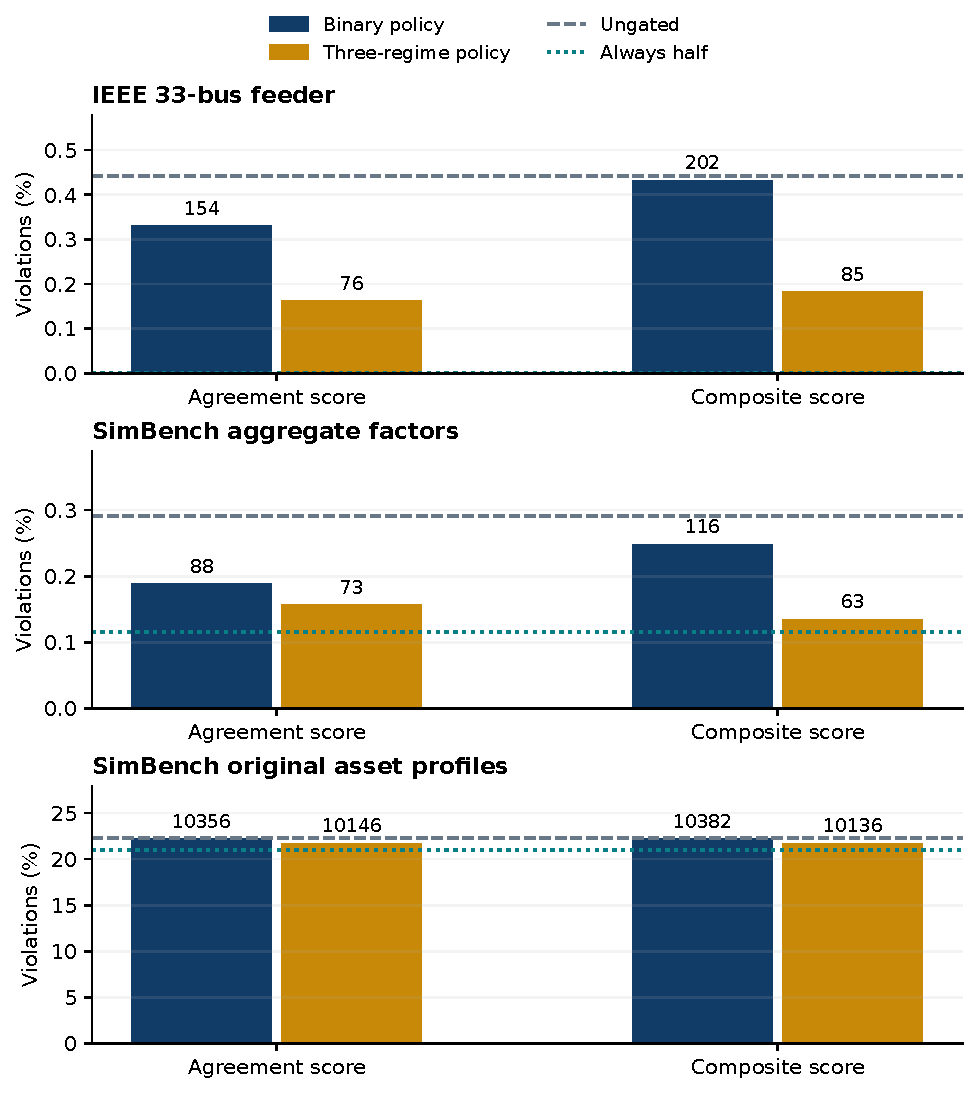
\includegraphics[width=.87\linewidth]{epsr_figures/Figure_2.pdf}
\caption{Score-policy comparisons across the three operating representations. Bars show agreement and composite scores under binary and three-regime policies. Horizontal lines show ungated and always-half dispatch. Labels give observed violating hours out of 46,656 hours per controller.}\label{fig:results2}
\end{figure}
Table~\ref{tab:paired} gives paired block uncertainty for the principal comparisons. Differences are left controller minus right controller; a negative violation difference indicates fewer failures. Composite three-regime gating has a negative interval against ungated dispatch in all three cases. Its asset-profile cost difference has an interval spanning zero. In contrast, its comparisons with agreement three-regime gating do not establish a consistent physical advantage. Composite binary gating increases the aggregate cases' violation rates relative to agreement binary gating. The supplementary paired tables include cost, network loss and non-zero activity for all prespecified comparisons.

\subsection{Condition dependence and retained battery operation}
Figure~\ref{fig:results3} disaggregates the stress-study mixture. Failures in the aggregate networks remain sparse, while the asset-profile case experiences sustained voltage excursions across several conditions. Reference outage and common bias test distinct assumptions: outage forces reference-dependent gates to hold, whereas common bias can preserve agreement despite incorrect operating factors. The reference-fed predictor and stress screen do not produce a common performance ordering across the networks. For example, the stress screen records 29 IEEE failures but 121 aggregate MV failures, compared with 0 and 54 under always-half operation. The finite perturbations provide no uniform protection across networks.


\clearpage\begin{landscape}
\begin{figure}[p]
\centering
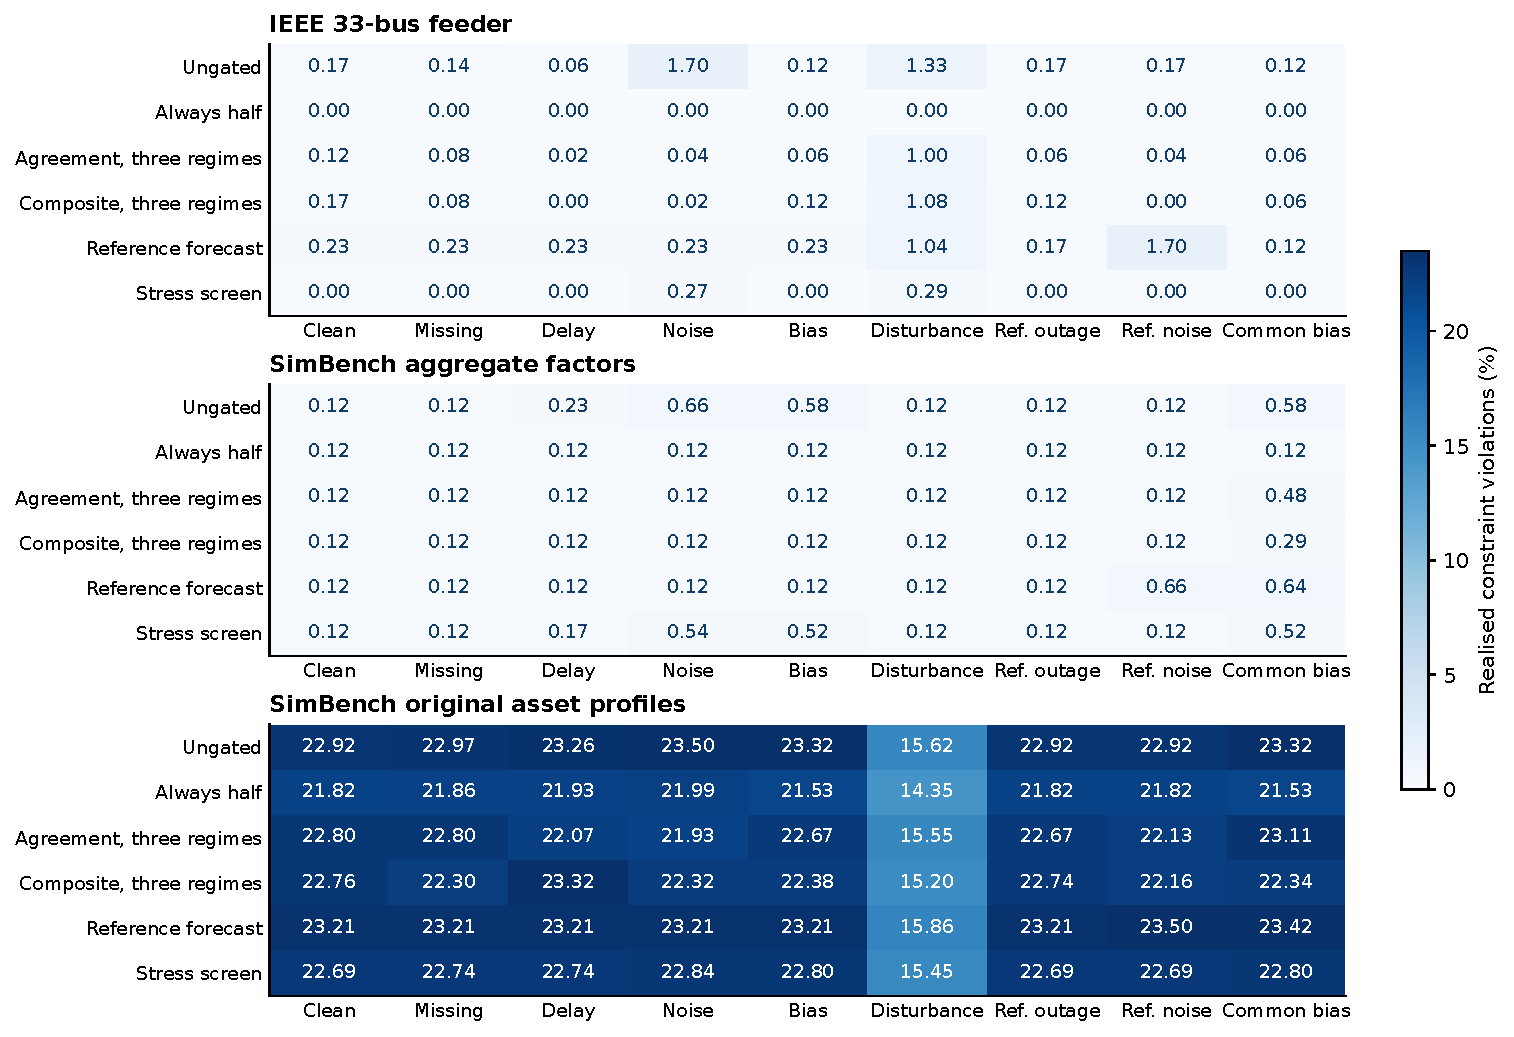
\includegraphics[width=245mm,height=155mm,keepaspectratio]{epsr_figures/Figure_3.pdf}
\caption{Violation percentages across nine measurement and operating conditions. Conditions and seeds are pooled with their prescribed equal weights over the twenty-four temporal blocks. A common colour scale is used across panels; printed values resolve the small aggregate-network rates. All issued actions, including holds, enter each denominator.}\label{fig:results3}
\end{figure}
\end{landscape}
\begin{table}[tbp]
\centering\small\setlength{\tabcolsep}{3.5pt}
\caption{Paired controller differences and 95\% stratified block-bootstrap intervals.}\label{tab:paired}
\begin{tabular}{llrr}
\toprule
Comparison & Representation & Violation difference (pp) & Cost difference (EUR)\\\midrule
T3 minus ungated & IEEE 33 & -0.259 [-0.369, -0.165] & +26.22 [+15.24, +37.07]\\
T3 minus ungated & MV aggregate & -0.156 [-0.261, -0.064] & +138.83 [+92.51, +185.49]\\
T3 minus ungated & MV asset profiles & -0.581 [-0.892, -0.302] & +25.08 [-16.92, +65.04]\\
T3 minus A3 & IEEE 33 & +0.019 [-0.028, +0.066] & +9.67 [+4.48, +14.92]\\
T3 minus A3 & MV aggregate & -0.021 [-0.049, +0.000] & +43.97 [+30.93, +57.55]\\
T3 minus A3 & MV asset profiles & -0.021 [-0.223, +0.176] & +25.58 [-3.30, +51.02]\\
T2 minus A2 & IEEE 33 & +0.103 [+0.056, +0.154] & +15.96 [+9.10, +23.47]\\
T2 minus A2 & MV aggregate & +0.060 [+0.011, +0.118] & +56.26 [+39.20, +73.74]\\
T2 minus A2 & MV asset profiles & +0.056 [-0.039, +0.154] & +66.69 [+45.84, +89.58]\\
T3 minus half & IEEE 33 & +0.182 [+0.107, +0.268] & +45.97 [+29.17, +63.51]\\
T3 minus half & MV aggregate & +0.019 [+0.000, +0.049] & +21.12 [+2.97, +40.69]\\
T3 minus half & MV asset profiles & +0.765 [+0.407, +1.172] & +81.71 [+42.30, +118.69]\\
\bottomrule\end{tabular}
\par\smallskip\parbox{\linewidth}{\footnotesize A and T denote agreement and composite evidence. Numerals 2 and 3 denote binary and three-regime policies. The bootstrap retains all conditions and measurement seeds within each of twenty-four physical blocks. Intervals are conditional on the benchmark design; multiple contrasts are descriptive rather than multiplicity-adjusted hypothesis tests.}
\end{table}
\begin{table}[tbp]
\centering\small\setlength{\tabcolsep}{3.5pt}
\caption{Authorisation, delivered activity and mean network loss per 72-hour block.}\label{tab:activity}
\begin{tabular}{lrrrr}
\toprule
Representation & Controller & Authorised (\%) & Non-zero (\%) & Loss (MWh)\\\midrule
IEEE 33 & Ungated & 100.00 & 39.14 & 0.757\\
IEEE 33 & Always half & 100.00 & 62.52 & 0.509\\
IEEE 33 & Agreement (3) & 83.00 & 40.70 & 0.630\\
IEEE 33 & Composite (3) & 83.08 & 41.08 & 0.610\\
MV aggregate & Ungated & 100.00 & 16.75 & 3.833\\
MV aggregate & Always half & 100.00 & 26.69 & 3.641\\
MV aggregate & Agreement (3) & 83.00 & 18.27 & 3.736\\
MV aggregate & Composite (3) & 83.08 & 18.10 & 3.730\\
MV asset profiles & Ungated & 100.00 & 21.65 & 5.493\\
MV asset profiles & Always half & 100.00 & 36.72 & 5.309\\
MV asset profiles & Agreement (3) & 83.30 & 24.18 & 5.405\\
MV asset profiles & Composite (3) & 82.74 & 23.47 & 5.405\\
\bottomrule\end{tabular}
\end{table}
Table~\ref{tab:activity} shows why authorisation and useful battery operation must be distinguished. Ungated operation permits every recommendation, yet only 39.14\% of IEEE epochs issue non-zero power. Always-half operation has 62.52\% non-zero activity in the same case. Its smaller commands retain energy for more later decisions, although individual support magnitudes are lower. The composite gate issues non-zero power in 41.08\%, 18.10\% and 23.47\% of IEEE, aggregate MV and asset-profile epochs, respectively. Different trajectories therefore affect both the availability of future actions and the network outcomes of a gate.

The stored-energy sensitivity retains each recorded trajectory and changes only its terminal valuation. The complete 90, 130 and 170~EUR/MWh cost tables are supplied in the supplement. This calculation exposes the dependence of reported economic comparisons on remaining energy. It supplies an accounting sensitivity, while dispatch under different tariff or valuation choices requires new optimisation runs.

\subsection{Score information and channel removal}
Figure~\ref{fig:results4} compares agreement and composite rankings on the same ungated proposals. Each representation supplies 40,608 degraded-condition proposals with a current reference. At 50\% coverage, composite and agreement risks are 0.443\% and 0.364\% for IEEE, 0.167\% and 0.207\% for aggregate MV, and 17.711\% and 21.218\% for asset profiles. At 75\% coverage, the composite retains an asset-profile advantage, with risk 20.265\% against 21.306\%. At 90\%, that ordering disappears: the respective risks are 21.674\% and 21.550\%. Aggregate MV also changes ordering as coverage rises. These are finite-set ranking results on common proposals, not operating trajectories produced by test-fitted thresholds.

\begin{figure}[p]
\centering
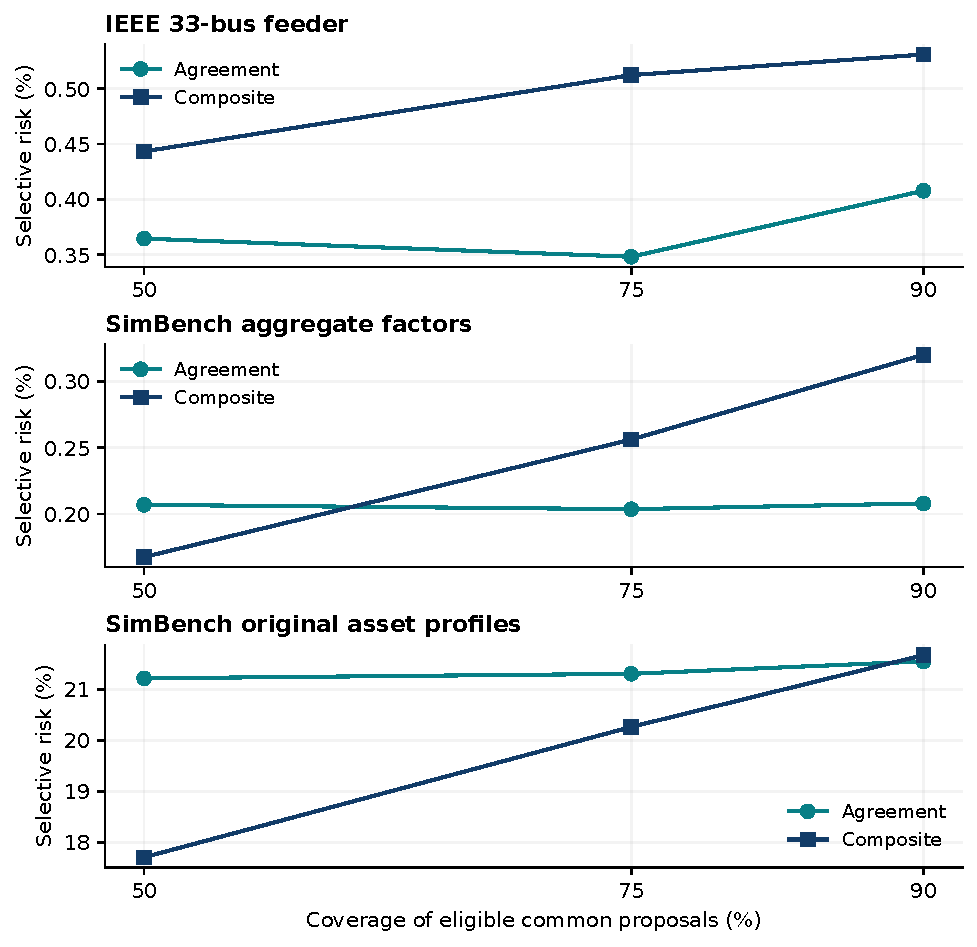
\includegraphics[width=.82\linewidth]{epsr_figures/Figure_4.pdf}
\caption{Selective physical risk of identical ungated proposals ranked by agreement and composite evidence. Selection retains 50\%, 75\% and approximately 90\% of the same eligible proposals. Every score uses the same proposal, state of charge and realised outcome; the selection order uses only the score and an outcome-independent tie order.}\label{fig:results4}
\end{figure}
\begin{table}[tbp]
\centering\small\setlength{\tabcolsep}{3.5pt}
\caption{Channel-removal controls with renormalised weights and separately calibrated development cutoffs.}\label{tab:ablations}
\begin{tabular}{lrrrrrr}
\toprule
Three-regime score & IEEE (\%) & MV (\%) & Asset (\%) & IEEE (EUR) & MV (EUR) & Asset (EUR)\\\midrule
Composite (3) & 0.182 & 0.135 & 21.725 & 4861.54 & 777.18 & 1097.73\\
Without freshness & 0.182 & 0.133 & 21.569 & 4856.52 & 759.55 & 1064.97\\
Without completeness & 0.171 & 0.129 & 21.701 & 4861.08 & 779.28 & 1099.79\\
Without maturity & 0.182 & 0.159 & 21.806 & 4866.56 & 771.29 & 1114.67\\
Without agreement & 0.193 & 0.133 & 21.646 & 4864.88 & 793.18 & 1101.79\\
\bottomrule\end{tabular}
\end{table}
The channel-removal results in Table~\ref{tab:ablations} also vary by representation. Removing completed forecast performance leaves the IEEE violation count unchanged at 85, while increasing aggregate MV failures from 63 to 74 and asset-profile failures from 10,136 to 10,174. Removing freshness lowers asset-profile failures to 10,063 and mean cost to EUR~1,064.97. Removing agreement gives 90 IEEE failures, 62 aggregate MV failures and 10,099 asset-profile failures. No individual removal worsens every physical and economic outcome. Because removal also changes the score distribution and fitted cutoffs, these comparisons assess complete retained-channel policies rather than a derivative of one fixed threshold. The full score consequently has conditional information value, with no uniform superiority established by this design.

\subsection{Violation severity, duration and available alternatives}
All observed failures are voltage violations. IEEE failures are under-voltage events, and SimBench failures are over-voltage events. No thermal limit is crossed in the executed test records. Table~\ref{tab:physical} reports extrema, affected bus-hours and longest within-block failure runs. Asset-profile events extend to 55 consecutive hours, compared with at most four hours on IEEE and two hours in aggregate MV operation. The sustained asset events therefore cannot be described as occasional misclassification of an otherwise benign network state.

\begin{table}[tbp]
\centering\small\setlength{\tabcolsep}{3.5pt}
\caption{Realised voltage extrema and extent of observed limit violations.}\label{tab:physical}
\begin{tabular}{lrrrrr}
\toprule
Representation & Controller & $V_{\min}$ (p.u.) & $V_{\max}$ (p.u.) & Longest (h) & Bus-hours\\\midrule
IEEE 33 & Ungated & 0.9367 & 1.0485 & 4 & 260\\
IEEE 33 & Always half & 0.9616 & 1.0281 & 0 & 0\\
IEEE 33 & Composite (3) & 0.9367 & 1.0387 & 4 & 114\\
MV aggregate & Ungated & 1.0033 & 1.0542 & 2 & 171\\
MV aggregate & Always half & 1.0033 & 1.0504 & 1 & 54\\
MV aggregate & Composite (3) & 1.0033 & 1.0533 & 2 & 70\\
MV asset profiles & Ungated & 1.0029 & 1.0622 & 55 & 19555\\
MV asset profiles & Always half & 1.0047 & 1.0622 & 55 & 18474\\
MV asset profiles & Composite (3) & 1.0029 & 1.0622 & 55 & 19120\\
\bottomrule\end{tabular}
\par\smallskip\parbox{\linewidth}{\footnotesize Bus-hours sum affected under-voltage and over-voltage buses over all 46,656 epochs. Longest duration is the maximum uninterrupted failure run within a 72-hour block. Extrema are taken over all buses and evaluated hours.}
\end{table}
The retrospective AC diagnostic evaluates thirteen power levels in each of 6,912 unique realised network states. Every state has at least one physically feasible tested power when energy bounds are ignored. This finding rules out an empty tested action set as the explanation for the observed failures. Energy capability on the recorded controller trajectory gives a different result. For composite gating with asset profiles, 6,610 of its 10,136 failures, or 65.21\%, have no energy-admissible feasible tested action. The remaining 3,526 failures have an available alternative at the same state of charge. Ungated operation has 8,186 energy-limited failures and 2,221 failures with an available alternative. Always-half operation has 6,943 and 2,836, respectively.

\begin{table}[tbp]
\centering\small\setlength{\tabcolsep}{3.5pt}
\caption{Retrospective failure partition on recorded battery trajectories.}\label{tab:feasibility}
\begin{tabular}{lrrrr}
\toprule
Representation & Controller & Failures & Energy-limited & Alternative exists\\\midrule
IEEE 33 & Ungated & 206 & 0 & 206\\
IEEE 33 & Always half & 0 & 0 & 0\\
IEEE 33 & Composite (3) & 85 & 0 & 85\\
MV aggregate & Ungated & 136 & 0 & 136\\
MV aggregate & Always half & 54 & 0 & 54\\
MV aggregate & Composite (3) & 63 & 0 & 63\\
MV asset profiles & Ungated & 10407 & 8186 & 2221\\
MV asset profiles & Always half & 9779 & 6943 & 2836\\
MV asset profiles & Composite (3) & 10136 & 6610 & 3526\\
\bottomrule\end{tabular}
\par\smallskip\parbox{\linewidth}{\footnotesize Every realised state has a feasible power among the thirteen tested levels before energy screening, so the no-feasible-power category is zero throughout. Alternative exists means at least one tested AC-feasible level satisfies the recorded battery energy bounds. It does not construct an alternative multi-hour trajectory.}
\end{table}
For IEEE, every failure has an energy-admissible feasible alternative among the tested levels. Composite gating has the same property in aggregate MV operation; fourteen agreement three-regime failures in that case are energy-limited. With asset profiles, the composite controller records 8,209 forecast-infeasible zero commands, of which 7,364 also violate the realised network limits. The model therefore often identifies an estimated state in which the implemented candidate and energy constraints provide no acceptable recommendation. Issuing a logged zero command preserves the decision record, but cannot restore a feasible network state by itself.

Figure~\ref{fig:results5} provides the prespecified noisy asset-profile block beginning on 1 November with seed 11. Voltage, command and state-of-charge traces link the hourly outcomes to the battery trajectory. The illustration complements the complete event counts and the fixed-trajectory action diagnostic. Together they locate the principal remaining design need: preserving energy headroom for later voltage support, while correcting forecasts and action choices in hours where an admissible alternative already exists.

\begin{figure}[p]
\centering
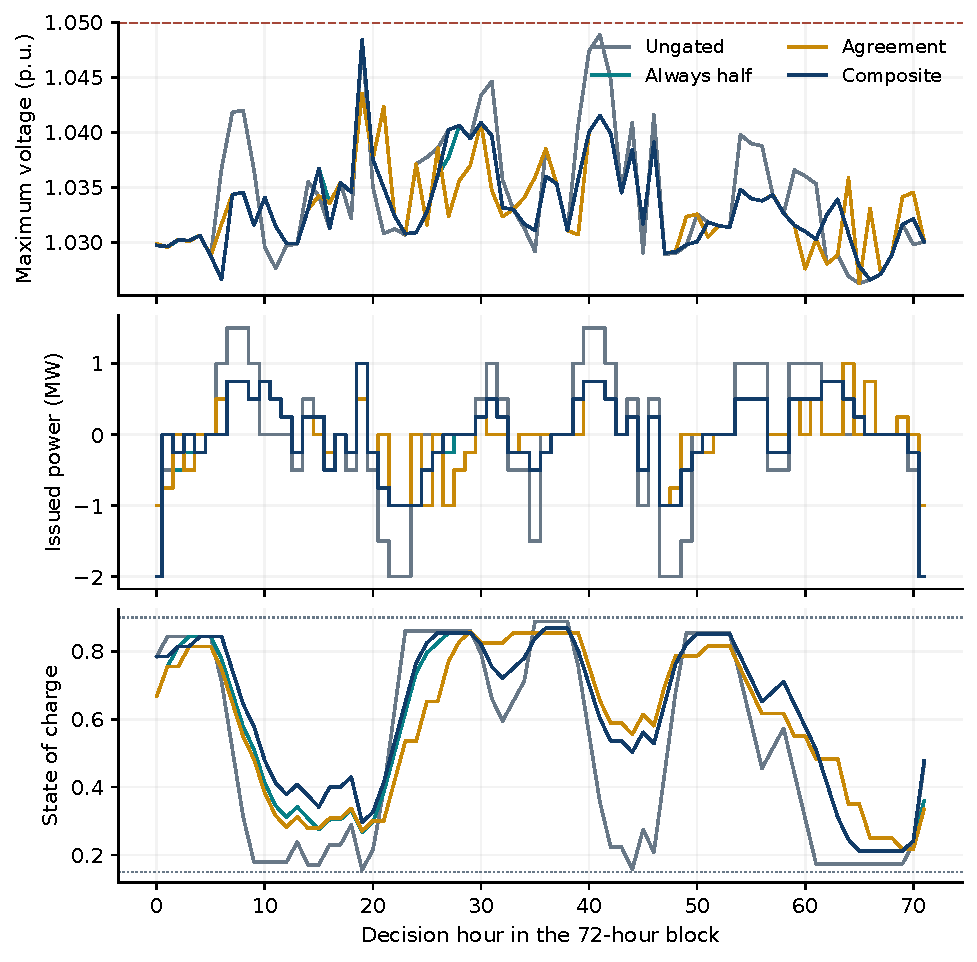
\includegraphics[width=.94\linewidth]{epsr_figures/Figure_5.pdf}
\caption{Prespecified illustrative block: SimBench asset profiles, noisy primary measurements, 1 November start, seed 11. Panels show realised maximum bus voltage, issued battery power and state of charge for ungated, always-half, agreement three-regime and composite three-regime dispatch. Voltage limits and battery bounds are shown for context. The trace is an illustration of one block, while Tables~
ef{tab:overall} and 
ef{tab:feasibility} use the complete study.}\label{fig:results5}
\end{figure}
\section{Discussion}\label{sec:discussion}
The controlled comparisons identify two sources of operating behaviour: the evidence used to select a regime and the power restriction applied within that regime. Their effects depend on the battery trajectory and the spatial representation of the network. This dependence provides the basis for interpreting the proposed gate as a supervisory component with a measurable operating trade-off.

\subsection{Information quality and action restriction}
The composite three-regime gate reduces failures relative to ungated dispatch in all three representations, but its comparison with always-half dispatch shows that evidence scoring is not required to obtain that ordering. Always-half dispatch has both lower observed failure rates and lower energy-adjusted cost under the tested objective. Agreement and composite scores also give different rankings under binary and three-regime policies. Thus a gate's benefit should be assessed against the same action restriction before it is attributed to richer measurement evidence.

Common-proposal ranking supplies a narrower result. Composite evidence distinguishes lower-risk asset-profile proposals better than agreement at 50\% and 75\% coverage, but this advantage disappears near 90\%. The deployed composite and agreement three-regime trajectories remain physically similar within the paired block intervals. Evidence can therefore contain useful selection information without producing a consistent improvement after state-dependent battery dispatch. The selection finding is conditional on coverage, representation and the specified mixture of faults.

The channel-removal controls likewise do not support a universal need for all four components at the chosen weights. The fixed weights supply an interpretable bounded indicator, while the outcomes show that they are not an optimal allocation of evidence for every network. A deployment-specific choice would require a separate development objective, followed by a frozen evaluation on new periods. Its objective should include delivered power, physical severity and economic cost, rather than increasing the number of indicators or authorisation percentage alone.

\subsection{Spatial operating states and energy headroom}
Replacing common aggregate factors with original asset profiles changes both the nodal inputs and the dimensional forecast task. Asset-profile operation has much higher over-voltage exposure and longer events than aggregate operation on the same SimBench electrical network. Because profile-coordinate noise also changes the variance of aggregate observations, this is evidence about the full operating representation rather than an isolated causal estimate of spatial diversity. Nevertheless, the difference shows that favourable aggregate-factor results cannot establish comparable performance for the supplied asset trajectories.

The realised-action diagnostic narrows the physical interpretation. Every tested state admits a feasible power level before energy screening. The dominant restriction in the asset case is the remaining storage headroom on the actual trajectory. Over-voltage mitigation can require absorption when the battery is already near its upper energy limit. A one-hour objective with a linear stored-energy value does not plan that headroom across a prolonged injection episode. The greater activity of always-half dispatch on IEEE further shows how reducing the present command can retain later options.

These findings connect the supervisory gate to the uncertainty-mitigation and voltage-flexibility problems studied by Sharma et al. \cite{sharma} and Gadari and Kiran \cite{gadari}. A useful extension is a multi-period dispatch kernel that reserves absorption and discharge capability for forecast network stress. Reactive support, curtailment and coordinated storage would expand the feasible control set. Such extensions need new operating comparisons because changing one hour's action changes the later battery trajectory. The retrospective counts identify feasible same-hour alternatives, but cannot be read as the number of failures eliminated by an implementable replacement policy.

\subsection{Reference reliability and uncertainty treatment}
The reference is valuable only within its reliability assumptions. Its outage reduces evidence-gate activity, while common bias can preserve meter agreement despite incorrect plant representation. Completed performance is also assessed against that reference, so common corruption affects more than one evidence channel. Reference-fed forecasting tests direct use of the additional observation stream and performs differently across representations. A more accurate current meter does not remove the next-hour prediction error or the dispatch kernel's energy limitation.

Finite-state stress screening achieves the lowest non-zero IEEE failure count among the forecast-based variants, yet its aggregate MV failure count exceeds those of both three-regime gates and always-half dispatch. Four jointly signed perturbations are a reproducible caution mechanism, but do not represent all spatial forecast errors. Joint residual coverage is also evaluated empirically and varies by season. For network protection, these statistical and scenario indicators must remain distinct from a validated robust or chance-constrained feasible set.

\subsection{Scope of the operating evidence}
The study uses balanced hourly AC models with fixed topology, one active-power-controlled battery, benchmark profiles and prescribed measurement faults. Field communication effects, topology errors, unbalanced phases, converter transients and corrupted battery-state measurements are outside this assessment. Voltage limits and tariffs are imposed study settings. IEEE line-current ratings are also assumed, and the executed periods do not establish behaviour under binding thermal constraints. More networks, years, battery locations and fault mechanisms are needed to assess transfer beyond these cases.

The twenty-four temporal blocks improve seasonal coverage while retaining dependence within each block. The stratified intervals quantify variation across those sampled periods. They do not turn measurement seeds or correlated controller records into independent field observations. Equal fault weighting gives a controlled stress comparison rather than a forecast of operational fault frequency. Within these limits, the saved inputs, source version, command records and independent numerical checks make the evidence inspectable and reproducible.

\section{Conclusion}\label{sec:conclusion}
A causal evidence gate has been formulated and evaluated for hourly battery dispatch under degraded measurements. It combines observation age, availability, completed forecast performance and meter agreement, then checks the chosen command against the predicted AC network state. Fourteen configurations, two rolling forecast origins and twenty-four temporal blocks separate evidence scoring from action restriction and test reference reliability and spatial operating profiles.

Composite three-regime gating reduces failures relative to ungated dispatch in every tested representation, with higher mean energy-adjusted cost. Always-half dispatch gives lower observed failure rates and lower cost than that gate in all three cases. Composite evidence improves common-proposal selection over agreement only at selected coverage levels in the asset-profile case, while channel removal yields no uniform ordering. These comparisons establish conditional operating value rather than general superiority of the composite score.

The asset-profile case reveals the principal control limitation. A feasible tested power exists in every realised state before energy screening, but battery bounds exclude all such powers during 65.21\% of composite-gate failures. Future work should connect causal evidence to multi-period energy-headroom management and assess wider network and control configurations. The present archive supplies a reproducible basis for those comparisons and for testing whether additional information produces a useful physical improvement after its action policy is held explicit.

\section*{Data and code availability}
The executed study, input profiles, editable figure sources and Python implementation are available in the versioned project archive \cite{software}. The \href{https://github.com/Devchandrasen/tudt-f-smart-energy/releases/tag/v3.0.0}{v3.0.0 release} supplies the complete per-hour numerical archive and SHA-256 manifest. Supplementary material provides all controller summaries, chronological configuration, paired uncertainty and numerical validation records. SimBench-derived data retain the original database terms documented with the archive \cite{dataset}. The 2016 benchmark profiles and simulated faults can be reproduced without access to private field measurements.

\appendix
\section{Implementation and numerical checks}\label{sec:checks}
The arithmetic audit covers all 1,959,552 controller records. Battery updates agree with Eq.~\eqref{eq:soc} to a maximum absolute error of $1.11\times10^{-16}$. No proposal or issued command violates the battery bounds, and no non-zero issued command fails its recorded forecast-state AC check. Regime reconstruction, reference fallback and realised-feasibility labels have zero disagreements. The maximum command-rule error is $5.55\times10^{-17}$~MW and the score reconstruction error is $3.33\times10^{-16}$.

Fresh uncached solves check 114 realised states and 114 forecast-command pairs, including sampled and failed outcomes across both origins and all three representations. Their feasibility labels agree with the archive. The maximum difference in the checked physical metrics is $6.25\times10^{-8}$. The retrospective action audit finds no feasible issued command excluded from its energy-admissible set, and the three failure categories partition every controller's recorded failures exactly.

Twenty-nine automated tests cover causal information timing, battery and command rules, development partitions, reference handling and historical archive integrity. A profile-mapping check compares every supplied load's active and reactive values and every generator's active value over all 8,784 hours with the official SimBench conversion. Agreement is within $10^{-12}$. These checks support implementation consistency; the operational conclusions remain conditional on the model and experimental design described above.


\begin{thebibliography}{99}
\bibitem{ardebili} A. Aghazadeh Ardebili, M. Zappatore, A.I.H.A. Ramadan, A. Longo, A. Ficarella, Digital Twins of smart energy systems: a systematic literature review on enablers, design, management and computational challenges, Energy Informatics 7 (2024) 94. \href{https://doi.org/10.1186/s42162-024-00385-5}{doi:10.1186/s42162-024-00385-5}.
\bibitem{hueros} P.J. Hueros-Barrios, J. Espolio-Maestro, S. Rodr\'iguez-Carrasco, C. Santos-P\'erez, F.J. Rodr\'iguez-S\'anchez, P. Mart\'in S\'anchez, M. Tradacete-\'Agreda, F. Blaabjerg, Real-time digital twin prototype for cyber-physical analysis of anomalies in PV-PEM-BESS systems for green hydrogen production, Sustainable Energy, Grids and Networks 45 (2026) 102152. \href{https://doi.org/10.1016/j.segan.2026.102152}{doi:10.1016/j.segan.2026.102152}.
\bibitem{bragatto} T. Bragatto, M.A. Bucarelli, F. Carere, M. Cresta, F.M. Gatta, A. Geri, M. Maccioni, M. Paulucci, P. Poursoltan, F. Santori, Near real-time analysis of active distribution networks in a Digital Twin framework: A real case study, Sustainable Energy, Grids and Networks 35 (2023) 101128. \href{https://doi.org/10.1016/j.segan.2023.101128}{doi:10.1016/j.segan.2023.101128}.
\bibitem{muhsen} H. Muhsen, A. Allahham, A. Al-Halhouli, M. Qandil, A digital twin framework for flexibility management using electric vehicle aggregators with embedded cyber-attack detection, Sustainable Energy, Grids and Networks 46 (2026) 102307. \href{https://doi.org/10.1016/j.segan.2026.102307}{doi:10.1016/j.segan.2026.102307}.
\bibitem{zhang} X. Zhang, D.K.J. Lin, L. Wang, Digital twin optimization: A sequential approach, Computers \& Industrial Engineering 208 (2025) 111235. \href{https://doi.org/10.1016/j.cie.2025.111235}{doi:10.1016/j.cie.2025.111235}.
\bibitem{panda} S.P. Panda, B. Genest, A. Easwaran, R. Rigo-Mariani, P. Lin, Methods for mitigating uncertainty in real-time operations of a connected microgrid, Sustainable Energy, Grids and Networks 38 (2024) 101334. \href{https://doi.org/10.1016/j.segan.2024.101334}{doi:10.1016/j.segan.2024.101334}.
\bibitem{rahman} D.M. Rahman, S. Ganguly, Voltage regulation and energy loss minimization for distribution networks with high photovoltaic penetration and EV charging stations using dual-stage model predictive control, Sustainable Energy, Grids and Networks 40 (2024) 101529. \href{https://doi.org/10.1016/j.segan.2024.101529}{doi:10.1016/j.segan.2024.101529}.
\bibitem{khojasteh} M. Khojasteh, P. Faria, Z. Vale, Energy and reserve optimization in local energy communities using linear decision rules, Sustainable Energy, Grids and Networks 46 (2026) 102287. \href{https://doi.org/10.1016/j.segan.2026.102287}{doi:10.1016/j.segan.2026.102287}.
\bibitem{hou} Z.J. Hou, T. Fu, H. Ren, D. Wang, X. Ma, D. Wu, An uncertainty-informed Digital Twin framework for optimal long-duration energy storage dispatch, International Journal of Electrical Power \& Energy Systems 177 (2026) 111852. \href{https://doi.org/10.1016/j.ijepes.2026.111852}{doi:10.1016/j.ijepes.2026.111852}.
\bibitem{li} L. Li, Y. Ju, Z. Wang, Quantifying the impact of building load forecasts on optimizing energy storage systems, Energy and Buildings 307 (2024) 113913. \href{https://doi.org/10.1016/j.enbuild.2024.113913}{doi:10.1016/j.enbuild.2024.113913}.
\bibitem{sharma} S.B. Sharma, J.T. Lee, D.S. Callaway, Distributed battery dispatch for uncertainty mitigation in renewable microgrids, Electric Power Systems Research 235 (2024) 110671. \href{https://doi.org/10.1016/j.epsr.2024.110671}{doi:10.1016/j.epsr.2024.110671}.
\bibitem{gadari} S.K. Gadari, D. Kiran, Network topology-aware operational voltage flexibility provision for forecast errors, Electric Power Systems Research 242 (2025) 111413. \href{https://doi.org/10.1016/j.epsr.2025.111413}{doi:10.1016/j.epsr.2025.111413}.
\bibitem{elmachtoub} A.N. Elmachtoub, P. Grigas, Smart ``Predict, then Optimize'', Management Science 68 (1) (2022) 9-26. \href{https://doi.org/10.1287/mnsc.2020.3922}{doi:10.1287/mnsc.2020.3922}.
\bibitem{paredes} \'A. Paredes, J.-F. Toubeau, J.A. Aguado, F. Vall\'ee, On the participation of energy storage systems in reserve markets using Decision Focused Learning, Sustainable Energy, Grids and Networks 42 (2025) 101677. \href{https://doi.org/10.1016/j.segan.2025.101677}{doi:10.1016/j.segan.2025.101677}.
\bibitem{breiman} L. Breiman, Random forests, Machine Learning 45 (2001) 5-32. \href{https://doi.org/10.1023/A:1010933404324}{doi:10.1023/A:1010933404324}.
\bibitem{angelopoulos} A.N. Angelopoulos, S. Bates, Conformal prediction: A gentle introduction, Foundations and Trends in Machine Learning 16 (2023) 494-591. \href{https://doi.org/10.1561/2200000101}{doi:10.1561/2200000101}.
\bibitem{oliveira} R.I. Oliveira, P. Orenstein, T. Ramos, J.V. Romano, Split conformal prediction and non-exchangeable data, Journal of Machine Learning Research 25 (225) (2024) 1-38. \url{https://jmlr.org/papers/v25/23-1553.html}.
\bibitem{gibbs} I. Gibbs, E.J. Cand\`es, Conformal inference for online prediction with arbitrary distribution shifts, Journal of Machine Learning Research 25 (162) (2024) 1-36. \url{https://jmlr.org/papers/v25/22-1218.html}.
\bibitem{liu} Y. Liu, P. Ning, M.K. Reiter, False data injection attacks against state estimation in electric power grids, ACM Transactions on Information and System Security 14 (1) (2011) 1-33. \href{https://doi.org/10.1145/1952982.1952995}{doi:10.1145/1952982.1952995}.
\bibitem{pasqualetti} F. Pasqualetti, F. D\"orfler, F. Bullo, Attack detection and identification in cyber-physical systems, IEEE Transactions on Automatic Control 58 (2013) 2715-2729. \href{https://doi.org/10.1109/TAC.2013.2266831}{doi:10.1109/TAC.2013.2266831}.
\bibitem{shen} Z. Shen, P. Sun, F. Arra\~no-Vargas, G. Konstantinou, Anomalous data evaluation for reliable updates of trustworthy power system digital twins, Expert Systems with Applications 314 (2026) 131434. \href{https://doi.org/10.1016/j.eswa.2026.131434}{doi:10.1016/j.eswa.2026.131434}.
\bibitem{dongliu} D. Liu, S. Timmerman, Y. Xiang, E. Hosseini, P. Palensky, P.P. Vergara, A data-driven approach for topology correction in low voltage distribution networks with photovoltaics, Sustainable Energy, Grids and Networks 46 (2026) 102321. \href{https://doi.org/10.1016/j.segan.2026.102321}{doi:10.1016/j.segan.2026.102321}.
\bibitem{gao} P. Gao, G. Zhao, Y. Hu, Y. Li, R. Liu, Robust coupling impedance-based topology identification method for asynchronous low-voltage distribution networks, Sustainable Energy, Grids and Networks 47 (2026) 102509. \href{https://doi.org/10.1016/j.segan.2026.102509}{doi:10.1016/j.segan.2026.102509}.
\bibitem{geifman} Y. Geifman, R. El-Yaniv, Selective classification for deep neural networks, Advances in Neural Information Processing Systems 30 (2017) 4878-4887. \url{https://proceedings.neurips.cc/paper/7073-selective-classification-for-deep-neural-networks.pdf}.
\bibitem{baran} M.E. Baran, F.F. Wu, Network reconfiguration in distribution systems for loss reduction and load balancing, IEEE Transactions on Power Delivery 4 (1989) 1401-1407. \href{https://doi.org/10.1109/61.25627}{doi:10.1109/61.25627}.
\bibitem{meinecke} S. Meinecke, D. Sarajli\'c, S.R. Drauz, A. Klettke, L.-P. Lauven, C. Rehtanz, A. Moser, M. Braun, SimBench: A benchmark dataset of electric power systems to compare innovative solutions based on power flow analysis, Energies 13 (2020) 3290. \href{https://doi.org/10.3390/en13123290}{doi:10.3390/en13123290}.
\bibitem{thurner} L. Thurner, A. Scheidler, F. Sch\"afer, J.-H. Menke, J. Dollichon, F. Meier, S. Meinecke, M. Braun, pandapower: An open-source Python tool for convenient modeling, analysis, and optimization of electric power systems, IEEE Transactions on Power Systems 33 (2018) 6510-6521. \href{https://doi.org/10.1109/TPWRS.2018.2829021}{doi:10.1109/TPWRS.2018.2829021}.
\bibitem{dataset} [dataset] SimBench, Power-system benchmark data and 2016 operating profiles, case \texttt{1-MV-rural-{}-0-sw}, distributed with SimBench 1.6.3. \url{https://simbench.de/en/download/datasets/} (accessed 6 October 2026).
\bibitem{efron} B. Efron, Bootstrap methods: Another look at the jackknife, The Annals of Statistics 7 (1) (1979) 1-26. \href{https://doi.org/10.1214/aos/1176344552}{doi:10.1214/aos/1176344552}.
\bibitem{software} [software and data] C. Pandey, TUDT-F distribution-network dispatch benchmark, version 3.0.0 (2026). \url{https://github.com/Devchandrasen/tudt-f-smart-energy/releases/tag/v3.0.0} (accessed 11 October 2026).
\end{thebibliography}
\end{document}
